\documentclass[preprint,12pt]{elsarticle}

% ------------------------------------------------------------
% Manuscript prepared for Big Data Research (Elsevier)
% Authors: Dilshod A'zamjonov, Sejuti Rahman
% Compile: pdflatex x2 (bibliography is embedded; no BibTeX run needed)
% ------------------------------------------------------------

\usepackage[T1]{fontenc}
\usepackage[utf8]{inputenc}
\usepackage{lmodern}
\usepackage{amsmath}
\usepackage{amssymb}
\usepackage{booktabs}
\usepackage{graphicx}
\usepackage{multirow}
\usepackage{array}
\newcolumntype{L}[1]{>{\raggedright\arraybackslash}p{#1}}
\setlength{\emergencystretch}{1.5em}
\usepackage{threeparttable}
\usepackage{rotating}
\usepackage{tikz}
\usetikzlibrary{positioning,arrows.meta,shapes.geometric,calc,fit,backgrounds}
\usepackage{pgfplots}
\pgfplotsset{compat=1.18}
\usepgfplotslibrary{groupplots}
\PassOptionsToPackage{hyphens}{url}
\usepackage[hidelinks]{hyperref}
\usepackage{xurl}

\newcommand{\Kfeat}{K}
\newcommand{\AUC}{\mathrm{AUC}}
\newcommand{\KS}{\mathrm{KS}}
\newcommand{\PSI}{\mathrm{PSI}}
\newcommand{\TPR}{\mathrm{TPR}}
\newcommand{\FPR}{\mathrm{FPR}}

\journal{Big Data Research}

% ------------------------------------------------------------
% HIGHLIGHTS (upload as a separate file at submission; 85 characters max each)
%  - LLM-assisted feature selection beats the best classical selector in 5 of 6 OOT cases
%  - Paired out-of-time AUC gains of +0.012 to +0.051 survive Holm correction
%  - Home Credit logistic regression still favours mutual-information mRMR
%  - A CLIP-style feature representation gives reproducible, source-dependent rankings
%  - Rank voting beats sequential screening in 5 of 8 cases but not full-pool mRMR
% ------------------------------------------------------------

\begin{document}

\begin{frontmatter}

\title{Semantic Screening for Credit-Risk Feature Selection: Temporal Out-of-Time Evaluation, Subset Stability, and Cross-Dataset Representation Transfer}

\author[aff1]{Dilshod A'zamjonov\corref{cor1}}
\ead{dilshod1526@gmail.com}

\author[aff2]{Sejuti Rahman}
\ead{sejuti@gmail.com}

\cortext[cor1]{Corresponding author}

\address[aff1]{Department of Engineering, New Uzbekistan University, 1 Movarounnahr Street, Mirzo Ulugbek District, Tashkent, Uzbekistan}
\address[aff2]{Department of Computing, New Uzbekistan University, 1 Movarounnahr Street, Mirzo Ulugbek District, Tashkent, Uzbekistan}

\begin{abstract}
Credit-risk models are built from hundreds or thousands of engineered predictors, and selecting a compact subset must balance discrimination, redundancy, reproducibility and stability over time. This study asks whether large language models (LLMs) can screen such feature spaces from feature meaning alone, and how the resulting subsets compare with classical selectors under temporal validation. We evaluate fifteen selection strategies, spanning statistical filters, wrappers, embedded methods, pure LLM screening with GPT-4.1 mini, LLM--classical hybrids, a CLIP-style contrastive feature representation and rank voting, on three temporally split datasets (Home Credit, LendingClub and Home Credit Model Stability 2024) with logistic regression and CatBoost backbones and fixed budgets of 20 and 40 features. Every development decision is frozen before a single locked out-of-time evaluation. LLM-assisted selection attains significantly higher out-of-time ROC-AUC than the best classical comparator in five of six dataset--model cases, with paired differences between $+0.012$ and $+0.051$ after Holm correction, whereas Home Credit logistic regression favours mutual-information mRMR ($-0.021$). Selected subsets also exceed the full-feature reference in five of six cases. The contrastive representation produces reproducible fold-to-fold selections (Nogueira stability up to 0.7525) and transfers across datasets in a source-dependent manner, and parallel rank voting recovers information lost by sequential screening in five of eight cases without surpassing full-pool mRMR. The results position LLM screening as an effective first-pass semantic filter whose benefit depends on the dataset and the downstream model, and which should be governed jointly with stability and drift monitoring.
\end{abstract}

\begin{keyword}
Credit scoring \sep Feature selection \sep Large language models \sep Temporal validation \sep Selection stability \sep Contrastive representation \sep Rank aggregation
\end{keyword}

\end{frontmatter}

% ============================================================
% 1. INTRODUCTION
% ============================================================

\section{Introduction}
\label{sec:introduction}

Retail credit-risk models are increasingly built on large, heterogeneous feature universes. Application records are joined with bureau histories, previous-loan behaviour, instalment schedules and card or point-of-sale transactions, and each source table is aggregated at several depths and time windows. The result is a predictor space of hundreds to thousands of engineered variables in which many columns are redundant, some are unstable across time, and a few are not reliably available at the moment a lending decision is taken \cite{thomas2002,siddiqi2006,anderson2007}. Selecting a compact subset from such a space is therefore not a purely statistical exercise. A variable that is semantically plausible may be redundant or temporally fragile, while a statistically useful variable may have weak lineage or depend on information that arrives only after origination. In a regulated domain, the selected subset must also remain reproducible, monitorable and explainable throughout the life of the model \cite{lessmann2015,gunnarsson2021,ballegeer2025}.

Classical feature selection addresses these requirements from the data side. Filters rank variables by relevance and redundancy statistics such as information value or mutual information \cite{guyon2003,peng2005}; wrappers search subsets with a learning algorithm in the loop \cite{kohavi1997,guyon2002,kursa2010}; embedded methods obtain importance from the fitted model itself \cite{tibshirani1996,lundberg2017}. None of these methods reads the meaning of a feature name or a data-dictionary description. Large language models (LLMs) have recently been proposed as a complementary source of evidence: given feature names, descriptions and a task statement, an LLM can rank or select features without seeing a single training row, and such semantic priors have been shown to be competitive with data-driven selectors on generic benchmarks \cite{jeong2025,li2025sigkdd,zhang2025llmlasso,choi2022}. Separately, contrastive representation learning has shown that two views of the same object, for example an image and a caption, can be aligned in a shared embedding space \cite{radford2021,oord2018}. Applied to features rather than images, the same idea yields a representation in which textual descriptions and target-free statistical descriptors of a predictor are aligned, so that features can be ranked, compared and transferred between datasets without reference to outcomes.

Whether these semantic tools help credit scoring is an empirical question with several parts. First, does an LLM-screened subset discriminate at least as well as a classically selected one on later, out-of-time (OOT) data, under a fixed feature budget and a frozen development protocol? Second, are the selected subsets reproducible across development folds, given that reproducibility matters for governance independently of predictive performance \cite{kalousis2007,nogueira2018}? Third, does a feature representation learned on one lending portfolio transfer to another, and does a transferred ranking still support competitive downstream models? Fourth, is the usual sequential arrangement, in which semantic screening precedes statistical refinement, the right way to combine the two kinds of evidence, or does a parallel combination of rankings recover information that sequential screening discards? Existing LLM-selection studies address the first question on general-purpose benchmarks, and the stability literature addresses the second in the abstract, but the four questions have not been examined together in a temporally validated credit-risk setting with locked OOT evaluation.

This paper reports such an evaluation. We compare fifteen feature-selection strategies on three temporally split credit datasets: the Home Credit default-risk data, the LendingClub loan book, and the Home Credit Model Stability 2024 data, whose development population exceeds one million decisions \cite{homecredit2018,lendingclub_kaggle,homecredit2024}. Two model backbones, a penalised logistic regression and a gradient-boosted CatBoost model \cite{prokhorenkova2018}, are fitted on subsets of $\Kfeat=20$ and $\Kfeat=40$ original features respectively. Every ranking, subset, preprocessing map, hyperparameter and operating threshold is fixed on development data before the OOT window is opened once. The LLM component is GPT-4.1 mini \cite{openai2025gpt41} operating under two dataset-specific information contracts, one that receives training-only summary statistics and one that receives feature definitions and lineage only. The contrastive component is a CLIP-style feature representation trained on frozen development feature statistics and MiniLM text embeddings \cite{wang2020minilm,reimers2019}. The paper makes the following contributions.

\begin{enumerate}
    \item A temporally validated comparison of classical, model-based, LLM-assisted and representation-assisted feature selection across three credit datasets and two model backbones, with six prespecified paired OOT comparisons between the best LLM-assisted and the best classical selector in each dataset--model case.
    \item An explicit specification of the information each selection stage may consume, distinguishing target-free stages (LLM ranking, contrastive representation) from target-aware stages (information value, mRMR, Boruta, recursive elimination, model fitting), together with the leakage and freeze controls that separate development from OOT evaluation.
    \item A separation of four outcomes that are often conflated: downstream discrimination, fold-to-fold subset reproducibility measured by Nogueira stability and pairwise Jaccard similarity, distribution drift measured by score and feature population-stability indices, and feature-representation portability across datasets.
    \item A source-dependent contrastive-ranking extension, in which representations trained on three different portfolios rank the same 1,959 Stability predictors, and a Home Credit rank-voting experiment that tests parallel against sequential combination of semantic and statistical evidence.
    \item An account of the development of the protocol across successive experimental stages, documenting how the comparator set, the temporal split and the inference procedure changed and why.
\end{enumerate}

The remainder of the paper is organised as follows. Section~\ref{sec:related_work} reviews related work. Section~\ref{sec:background} provides background on credit-risk feature selection, classical selectors, semantic selection and selection stability. Section~\ref{sec:methodology} specifies the pipeline and each selection method. Section~\ref{sec:experimental_setup} describes the datasets, temporal design, models, metrics and inference. Section~\ref{sec:results} reports the results, Section~\ref{sec:discussion} discusses them, and Section~\ref{sec:conclusion} concludes. Appendices provide configuration details and supplementary results.


% ============================================================
% 2. RELATED WORK
% ============================================================

\section{Related Work}
\label{sec:related_work}

\paragraph{Credit-scoring benchmarks and feature selection}
Credit scoring has a long benchmarking tradition. Baesens et al.\ \cite{baesens2003} and Lessmann et al.\ \cite{lessmann2015} compared dozens of classifiers on multiple retail portfolios and established the practice of reporting several complementary metrics with statistical comparison across datasets; subsequent surveys catalogue the statistical and machine-learning models in use and the evaluation habits of the field \cite{louzada2016,dastile2020}, and Gunnarsson et al.\ \cite{gunnarsson2021} showed that gradient boosting remains a strong baseline against deep architectures on tabular credit data. Feature selection specifically for credit scoring has been studied from the predictive side, comparing filters and wrappers on public datasets \cite{laborda2021}, and from the business side, where the selected subset is optimised against expected profit and variable acquisition cost rather than accuracy alone \cite{maldonado2017,kozodoi2019}. These studies evaluate selectors on random or stratified splits and treat the selected subset as an input to a single classifier; they do not measure reproducibility of the subset across folds, drift of the selected variables over time, or the use of semantic information about the variables. Our study inherits their emphasis on multiple metrics and paired comparison but adds a locked OOT design and the stability and transfer outcomes.

\paragraph{Classical feature selection}
The filter, wrapper and embedded taxonomy of Kohavi and John \cite{kohavi1997} and Guyon and Elisseeff \cite{guyon2003} organises most classical work. Among filters, the minimum-redundancy maximum-relevance criterion of Peng et al.\ \cite{peng2005} selects features greedily by trading mutual information with the target against mutual information with already selected features; information-value ranking is the domain-specific filter of scorecard practice \cite{siddiqi2006,thomas2002}. Wrappers include recursive feature elimination \cite{guyon2002} and the Boruta procedure, which compares real features with permuted shadow copies inside a random forest \cite{kursa2010,breiman2001}. Embedded methods obtain relevance from the fitted model, through sparsity-inducing penalties \cite{tibshirani1996} or from additive attributions such as SHAP values \cite{lundberg2017}. Surveys from the data perspective \cite{li2017survey,saeys2007} and from the big-data perspective \cite{boloncanedo2015} note that scalability, redundancy handling and stability, rather than raw relevance ranking, dominate the practical difficulty in high-dimensional spaces. All classical selectors in this study are instances of these families and are fitted only on development folds.

\paragraph{Stability of feature selection}
Kalousis et al.\ \cite{kalousis2007} framed selection stability as robustness of the selected subset to perturbations of the training sample and proposed similarity-based measures; Kuncheva \cite{kuncheva2007} introduced a chance-corrected consistency index for fixed-size subsets; Nogueira et al.\ \cite{nogueira2018} unified these proposals in a statistical framework whose estimator is corrected for the size of the candidate universe and admits confidence intervals. Ensemble feature selection, which aggregates rankings from several selectors or resamples, was proposed as a route to more stable subsets \cite{saeys2008,boloncanedo2019}, and rank-aggregation methods studied for web search supply the aggregation rules \cite{dwork2001}. Ballegeer et al.\ \cite{ballegeer2025} recently examined the stability of post-hoc explanations in cost-sensitive credit scoring; that work concerns explanation stability after modelling, whereas we measure the stability of the selected subset before modelling. We report both Nogueira stability and mean pairwise Jaccard similarity and treat them as an outcome separate from discrimination.

\paragraph{Large language models for feature selection and engineering}
Choi et al.\ \cite{choi2022} showed that pre-trained language models encode usable task-specific priors over variables. Jeong et al.\ \cite{jeong2025} formalised LLM feature selection as scoring, ranking or sequential selection from feature names and a task description, and found GPT-4 selections competitive with LASSO and other data-driven baselines without access to training rows. Li et al.\ \cite{li2025sigkdd} contrasted data-driven and text-based LLM selection and identified conditions under which each works. Zhang et al.\ \cite{zhang2025llmlasso} used LLM-generated penalty factors to inform the LASSO penalty, and related work uses LLMs to engineer new features from dataset descriptions \cite{hollmann2023,han2024}. These methods are evaluated on general tabular benchmarks with random splits. Our contribution is to test the same class of semantic priors on credit portfolios under temporal validation, with dataset-specific information contracts that control exactly what metadata the model receives, and to evaluate the LLM both as a stand-alone selector and as the first stage of hybrids with statistical refinement.

\paragraph{Language models in credit risk}
Language models have entered credit-risk research mainly as extractors of predictive signal from borrower text. Sanz-Guerrero and Arroyo \cite{sanzguerrero2025} derive a risk indicator from peer-to-peer loan descriptions, and Xia et al.\ \cite{xia2025} combine LLM-extracted narrative variables with a boosted model under a tailored loss; Golec and AlabdulJalil \cite{golec2026} review the interpretability of LLM-based credit-risk systems. Those uses are distinct from ours: we do not extract borrower-level features from text, we use the language model to reason about the existing engineered feature universe, and borrower-level prediction remains the task of conventional classifiers trained on tabular data.

\paragraph{Contrastive representations and transfer}
CLIP \cite{radford2021} learns aligned image and text embeddings with an InfoNCE objective \cite{oord2018}; sentence encoders such as Sentence-BERT and MiniLM provide compact text embeddings for descriptions \cite{reimers2019,wang2020minilm}. We borrow the two-view alignment idea for features: the text view is the description of the feature and the statistical view is a vector of target-free descriptors computed on development data. The representation is used only to rank features, and its portability across portfolios is assessed with rank correlation \cite{spearman1904}, neighbourhood diagnostics \cite{venna2001,mcinnes2018} and, decisively, the downstream OOT performance of target-trained models.

\paragraph{Temporal validation and drift}
Random cross-validation overstates performance when data are ordered in time; blocked and expanding-window schemes are the appropriate alternative \cite{bergmeir2012}, and concept drift is the general phenomenon that makes later data differ from earlier data \cite{gama2014}. In credit risk the population stability index (PSI) is the standard monitoring statistic for distribution shift between development and later populations, and its statistical properties have been characterised only recently \cite{yurdakul2020}. The Home Credit Model Stability 2024 competition made temporal stability of discrimination an explicit objective \cite{homecredit2024}. Our design follows this literature: expanding-window development folds with a time gap, a single locked OOT window, and PSI reported for both model scores and selected features.

Taken together, prior work supplies selectors, stability measures, semantic priors and temporal evaluation designs, but no study evaluates LLM-assisted, contrastive and classical selection jointly on credit portfolios with locked OOT inference, fold-level stability and cross-dataset transfer. That joint evaluation is the gap addressed here.

% ============================================================
% 3. BACKGROUND
% ============================================================

\section{Background}
\label{sec:background}

\subsection{Credit-Risk Feature Selection}
\label{subsec:credit_risk_fs}

A retail credit model estimates the probability that an applicant or account experiences a defined adverse event within a horizon, using information available at the decision date. The engineered feature universe is typically assembled from several source tables: the application itself, external bureau records, the history of the applicant with the lender, and behavioural aggregates over rolling windows. Each source contributes variables at different depths (for example the most recent record, the mean over twelve months, or the count over the full history), so the universe contains strong within-source redundancy by construction. Feature selection in this setting has four requirements that are only partly aligned. Relevance to the outcome must be established on development data only. Redundancy should be limited, because redundant predictors inflate variance in logistic regression and complicate attribution. The selected subset should be reproducible, since a subset that changes with every refit is difficult to govern, document and explain to a validator. Finally, every retained variable must be available at decision time with a documented lineage, and its distribution should be stable enough between development and later populations that the model can be monitored with standard tools such as PSI \cite{siddiqi2006,thomas2002,yurdakul2020}.

These requirements motivate the evaluation design of this paper. Discrimination is measured out of time, because within-sample or randomly cross-validated estimates do not reveal temporal fragility \cite{bergmeir2012}. Reproducibility is measured across temporal development folds. Drift is measured for the model score and for each selected feature. Availability and lineage are enforced before selection, by restricting the candidate universe to approved raw predictors and by giving the language model access only to definitions and lineage in the dataset where such a review exists.

\subsection{Classical Feature Selection}
\label{subsec:classical_fs_background}

Let $X_1,\dots,X_d$ denote candidate features and $Y\in\{0,1\}$ the event indicator, with $Y=1$ for the adverse outcome. Classical selectors fall into three families \cite{kohavi1997,guyon2003}.

\emph{Filters} score features by a statistic computed from data alone and retain the top-ranked ones. The information value (IV) of scorecard practice bins a feature and compares the distribution of non-events and events across bins,
\begin{equation}
    \mathrm{WOE}_b=\ln\frac{g_b}{e_b},\qquad
    \mathrm{IV}=\sum_{b}(g_b-e_b)\,\mathrm{WOE}_b,
    \label{eq:iv}
\end{equation}
where $g_b$ and $e_b$ are the shares of non-events and events falling in bin $b$ and WOE is the weight of evidence \cite{siddiqi2006}. Mutual information $I(X_j;Y)$ is the general-purpose relevance statistic, and the minimum-redundancy maximum-relevance (mRMR) criterion \cite{peng2005} selects features greedily, adding at each step the feature that maximises relevance to the target minus its average redundancy with the set $S$ already selected,
\begin{equation}
    j^{\star}=\arg\max_{j\notin S}\Big[\,I(X_j;Y)-\frac{1}{|S|}\sum_{k\in S} I(X_j;X_k)\Big].
    \label{eq:mrmr}
\end{equation}
Mutual information between continuous variables is estimated with nearest-neighbour estimators \cite{kraskov2004,ross2014}. Principal component analysis is sometimes grouped with filters because it is unsupervised, but it replaces the original variables by orthogonal combinations rather than selecting them \cite{jolliffe2016}; its components are therefore not original features and need separate interpretation.

\emph{Wrappers} evaluate candidate subsets with a learning algorithm. Recursive feature elimination (RFE) fits a model, removes the least important feature or features, and repeats until the budget is reached \cite{guyon2002}. Boruta \cite{kursa2010} augments the data with shuffled shadow copies of every feature, fits a random forest \cite{breiman2001}, and iteratively confirms features whose importance is statistically higher than the best shadow importance, rejecting those that are not; it is an all-relevant procedure, so the confirmed set is then truncated to the budget.

\emph{Embedded} methods derive relevance from the model being fitted. Sparsity penalties zero out coefficients \cite{tibshirani1996}, and additive attribution methods such as SHAP \cite{lundberg2017} provide per-feature contribution magnitudes that can be aggregated over observations and used as a ranking. Because wrappers and embedded methods use the target, they must be fitted strictly inside development data, fold by fold, to avoid optimistic bias.

\subsection{Semantic / LLM-Assisted Selection}
\label{subsec:llm_fs_background}

Semantic selection uses information about what a feature \emph{is} rather than how it covaries with the target in the sample. Feature names, data-dictionary descriptions, source-table lineage, aggregation depth and logical type all carry information that an experienced credit analyst uses when reviewing a variable book, and this first-pass review is exactly the task delegated to the language model in this study. Jeong et al.\ \cite{jeong2025} showed that a capable LLM, prompted with feature names and a task description, produces importance scores or rankings that transfer to downstream models without any training rows; Li et al.\ \cite{li2025sigkdd} distinguished this text-based mode from data-driven modes in which the model is shown samples. The semantic prior can be used in three ways: directly, by taking the top-$\Kfeat$ ranked features as the subset (\emph{pure LLM}); as a screening stage that reduces the universe to a candidate pool later refined by a statistical selector (\emph{LLM then mRMR}, \emph{LLM then Boruta}); or as a completion mechanism that fills a statistically stable core up to the budget (\emph{stable core plus LLM fill}). In all three uses the LLM output is a fixed ranking that can be cached and reused, which makes the selection reproducible given the same model version, prompt and inputs, and inexpensive in tokens relative to the cost of model fitting.

Two properties of semantic selection matter for the evaluation. First, the LLM stage is target-free in the sense that it never sees outcomes, but a pipeline that contains it is not target-free as a whole if eligibility screening or downstream refinement uses development labels. Second, a fixed ranking reused across folds has trivially perfect fold agreement; its stability is therefore not comparable with that of selectors refitted in each fold, and the subset stability of LLM-assisted hybrids is inherited from the target-aware stage that follows the ranking.

A contrastive feature representation offers a different kind of semantic evidence. Following the two-view construction of CLIP \cite{radford2021}, each feature is described by a text view (its name and description, embedded with a sentence encoder \cite{reimers2019,wang2020minilm}) and a statistical view (a short vector of target-free descriptors such as missingness, dispersion and cardinality computed on development data). A small projection network is trained with an InfoNCE-type objective \cite{oord2018} so that the two views of the same feature are close and the views of different features are far apart, with the exception that verified identity-equivalent pairs are not treated as negatives. The learned space supports ranking features by similarity to a source anchor and, because the statistical view is target-free, the representation can be applied to the features of another dataset without refitting. Whether such a transferred ranking is useful can only be settled by training target-side models on the ranked subset and evaluating them out of time.

\subsection{Feature-Selection Stability}
\label{subsec:fs_stability_background}

Selection stability is the degree to which a selector returns the same subset when the training sample is perturbed \cite{kalousis2007}. For two selected sets $S_a$ and $S_b$ the Jaccard similarity $|S_a\cap S_b|/|S_a\cup S_b|$ \cite{jaccard1901} is the simplest measure, and averaging it over all unordered pairs of folds gives a mean pairwise Jaccard. Kuncheva \cite{kuncheva2007} corrected the overlap of fixed-size subsets for chance agreement, and Nogueira et al.\ \cite{nogueira2018} generalised the idea to a chance-corrected statistic defined on the matrix of selection indicators over a fixed candidate universe of size $d$, with an estimator that admits confidence intervals and hypothesis tests. Stability matters in credit risk for three reasons. A reproducible subset can be documented once and re-validated cheaply; large fold-to-fold changes signal that the selector is tracking sample noise rather than structure; and regulators and model validators expect the drivers of a score to be persistent. Stability is distinct from two other notions with which it is sometimes confused: population stability, which concerns the drift of the distribution of a variable over time and is measured by PSI, and explanation stability, which concerns the robustness of post-hoc attributions of a fitted model \cite{ballegeer2025}. This paper measures selection stability across five temporal development folds and reports it alongside, not instead of, discrimination and drift.

% ============================================================
% 4. METHODOLOGY
% ============================================================

\section{Methodology}
\label{sec:methodology}

\subsection{Overall Research Pipeline}
\label{subsec:pipeline}

Figure~\ref{fig:pipeline} summarises the pipeline. Its stages are executed in the following chronological order for every dataset.

\begin{enumerate}
    \item \textbf{Data assembly and outcome definition.} The engineered feature universe is assembled (529 predictors for Home Credit, 675 for LendingClub, 1,959 for Stability 2024) and the event definition of Section~\ref{subsec:datasets} is applied. For Stability 2024 a prediction-time availability review of 461 source variables approved 434 raw predictors and excluded 27; the 1,959 engineered features derive from the approved predictors.
    \item \textbf{Temporal split.} Each dataset is split by its time index into a development population (DEV) and a later, locked out-of-time population (OOT). OOT rows are set aside and are not touched again until the final scoring step.
    \item \textbf{Development folds.} DEV is divided into five expanding-window temporal folds with a time gap between the training and validation partitions of each fold; in Stability 2024 all decisions taken on the same date are kept in the same partition.
    \item \textbf{Eligibility and preprocessing.} Features with more than 95\% missing values are removed. For Home Credit and LendingClub an information-value eligibility interval of $0.01\le\mathrm{IV}\le0.50$ is applied before the LLM--statistical hybrids. Preprocessing maps (Section~\ref{subsec:preprocessing}) are fitted on the training partition of each fold.
    \item \textbf{Feature selection.} The fifteen strategies of Section~\ref{subsec:classical_fs}--\ref{subsec:voting_fs} produce a subset of original features of size $\Kfeat=20$ for logistic regression and $\Kfeat=40$ for CatBoost. Target-free rankings (the LLM ranking and the contrastive ranking) are computed once from metadata and development statistics and reused across folds; target-aware selectors are fitted on the training partition of each fold and applied to its validation partition without refitting.
    \item \textbf{Model fitting.} Logistic regression or CatBoost is fitted on the selected subset with the fixed configuration of Section~\ref{subsec:models}; final model encoding is applied after selection.
    \item \textbf{DEV validation.} Fold validation partitions yield discrimination estimates and the five fold-level subsets from which Nogueira stability and pairwise Jaccard similarity are computed.
    \item \textbf{Threshold selection.} Within each fold, the operating threshold that maximises the KS (Youden) separation $\TPR-\FPR$ on training scores is recorded; for the final model the threshold is derived from full-DEV training scores.
    \item \textbf{Freeze.} Final selectors, preprocessing maps and classifiers are refitted on full DEV. Feature rankings, retained subsets, model settings, operating thresholds and the DEV score-distribution bins used for PSI are then fixed and recorded in a pre-OOT manifest.
    \item \textbf{OOT scoring.} The frozen pipeline scores the OOT population once. ROC-AUC is the headline metric; KS, Brier score, Capture@10, PSI and threshold-dependent operating metrics are secondary. No retuning follows OOT scoring.
\end{enumerate}

Stages differ in the information they may consume. The LLM ranking and the contrastive representation are target-free: they receive feature metadata and, where the information contract allows it, training-only descriptive statistics, but never outcomes, validation statistics or OOT information. Domain rules, Random K and principal components are also target-free. Information value, mRMR, Boruta, recursive elimination, SHAP ranking, the stable-core construction, the redundancy stage after contrastive ranking, model fitting and threshold selection are target-aware and are confined to DEV training partitions. Leakage controls therefore operate at three levels: OOT exclusion from every development decision, fold-local fitting of every target-aware component, and hash-bound freezing of every artefact before the OOT population is opened.

\begin{figure}[htbp]
\centering
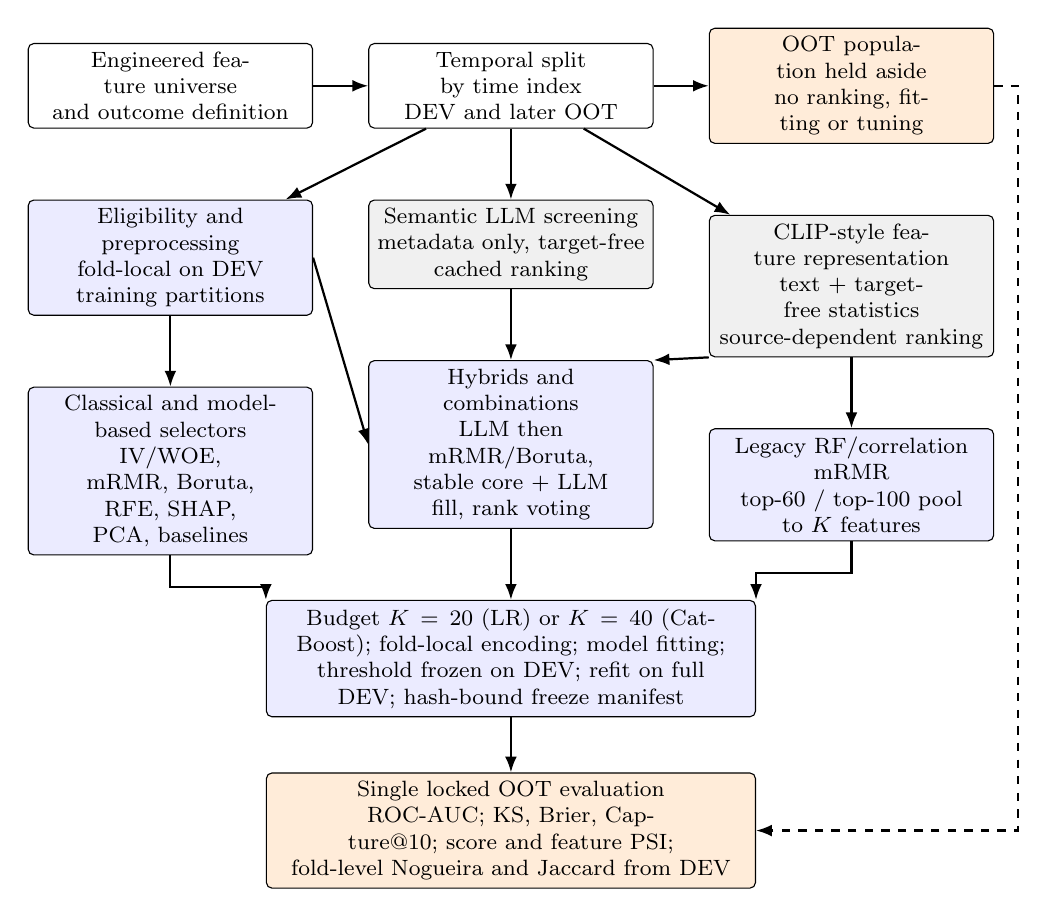
\begin{tikzpicture}[
    font=\footnotesize,
    node distance=5mm and 7mm,
    box/.style={draw, rounded corners=2pt, align=center, minimum height=9mm, inner sep=3pt, text width=34mm, fill=white},
    tfree/.style={box, fill=gray!12},
    taware/.style={box, fill=blue!8},
    oot/.style={box, fill=orange!15},
    arr/.style={-{Latex[length=2mm]}, thick},
    darr/.style={-{Latex[length=2mm]}, thick, dashed}
]
\node[box] (data) {Engineered feature universe\\and outcome definition};
\node[box, right=of data] (split) {Temporal split by time index\\DEV and later OOT};
\node[oot, right=of split] (ootheld) {OOT population held aside\\no ranking, fitting or tuning};

\node[taware, below=9mm of data] (elig) {Eligibility and preprocessing\\fold-local on DEV training partitions};
\node[tfree, below=9mm of split] (llm) {Semantic LLM screening\\metadata only, target-free\\cached ranking};
\node[tfree, below=9mm of ootheld] (clip) {CLIP-style feature representation\\text + target-free statistics\\source-dependent ranking};

\node[taware, below=9mm of elig] (classical) {Classical and model-based selectors\\IV/WOE, mRMR, Boruta,\\RFE, SHAP, PCA, baselines};
\node[taware, below=9mm of llm] (hybrid) {Hybrids and combinations\\LLM then mRMR/Boruta,\\stable core + LLM fill, rank voting};
\node[taware, below=9mm of clip] (legacy) {Legacy RF/correlation mRMR\\top-60 / top-100 pool\\to $K$ features};

\node[taware, below=9mm of hybrid, text width=60mm] (model) {Budget $K=20$ (LR) or $K=40$ (CatBoost); fold-local encoding; model fitting;\\threshold frozen on DEV; refit on full DEV; hash-bound freeze manifest};
\node[oot, below=7mm of model, text width=60mm] (eval) {Single locked OOT evaluation\\ROC-AUC; KS, Brier, Capture@10; score and feature PSI;\\fold-level Nogueira and Jaccard from DEV};

\draw[arr] (data) -- (split);
\draw[arr] (split) -- (ootheld);
\draw[arr] (split) -- (elig);
\draw[arr] (split) -- (llm);
\draw[arr] (split) -- (clip);
\draw[arr] (elig) -- (classical);
\draw[arr] (llm) -- (hybrid);
\draw[arr] (clip) -- (legacy);
\draw[arr] (elig.east) -- (hybrid.west);
\draw[arr] (clip.south west) -- (hybrid.north east);
\draw[arr] (classical.south) |- ++(0,-4mm) -| (model.north west);
\draw[arr] (hybrid) -- (model);
\draw[arr] (legacy.south) |- ++(0,-4mm) -| (model.north east);
\draw[arr] (model) -- (eval);
\draw[darr] (ootheld.east) -- ++(3mm,0) |- (eval.east);
\end{tikzpicture}
\caption{Research pipeline. Grey boxes are target-free stages, blue boxes are target-aware stages confined to development (DEV) training partitions, and orange boxes concern the locked out-of-time (OOT) population, which enters only at the final evaluation. Rank voting is a Home Credit experiment that averages the LLM and contrastive rankings before mutual-information mRMR.}
\label{fig:pipeline}
\end{figure}

\subsection{Data Preprocessing}
\label{subsec:preprocessing}

Numeric variables are processed by replacing infinite values with missing values, imputing missing values with the training-partition mean, and standardising to zero mean and unit variance with training-partition statistics. Categorical variables receive an explicit missing token and are one-hot encoded; levels unseen in the training partition are ignored, and rare levels are dropped below a minimum frequency of 10 observations for Home Credit and Stability 2024 and 50 observations for LendingClub. Home Credit and LendingClub matrices are held as dense single-precision arrays and Stability 2024 as a compressed sparse row matrix. Preprocessing maps are fitted on the training partition of each fold and, for the final model, on full DEV.

The order of operations is fixed. Eligibility screening and feature selection operate on \emph{original} features, with the selector receiving one numeric column per original candidate; a categorical variable is therefore selected or rejected as a whole. Final model encoding, including one-hot expansion, is performed only after the original-feature subset has been selected, so that the budget $\Kfeat$ counts original variables rather than encoded columns. Principal-component selection is the one exception: its retained quantities are components rather than original variables and are reported as such.

\subsection{Classical Feature-Selection Methods}
\label{subsec:classical_fs}

Table~\ref{tab:methods} lists the fifteen strategies. All target-aware selectors are fitted on the training partition of each fold using DEV labels only, then refitted on full DEV before OOT scoring. Unless stated otherwise the retained-feature rule is to rank the candidates by the method's own criterion and retain the top $\Kfeat$ original features. Implementation details not stated below are fixed in the public code repository listed in the Data availability statement.

\begin{table}[htbp]
\centering
\footnotesize
\begin{threeparttable}
\caption{Feature-selection strategies evaluated. The full-feature model is a reference and is excluded from selector comparisons.}
\label{tab:methods}
\begin{tabular}{@{}llL{58mm}@{}}
\toprule
Method & Family & Selection role \\
\midrule
Full features & Reference & No feature selection; context only. \\
Domain rules & Classical & Eligibility and policy filtering from credit-domain definitions. \\
Random K & Baseline & Random subset matched to the retained-feature budget. \\
PCA & Classical & Orthogonal components of the standardised candidates; components rather than original features. \\
IV/WOE & Classical & Stand-alone information-value ranking. \\
mRMR & Classical & Mutual-information relevance against mutual-information redundancy, Eq.~\eqref{eq:mrmr}. \\
Boruta RF & Classical & All-relevant random-forest wrapper with shadow-feature comparison. \\
IV then Boruta & Classical hybrid & Information-value pre-screen followed by Boruta confirmation. \\
RFE CatBoost & Model wrapper & Recursive elimination driven by CatBoost importance. \\
CatBoost SHAP & Embedded & Ranking by aggregated SHAP contribution magnitude. \\
Pure LLM & LLM-assisted & Direct semantic screening under the dataset-specific prompt contract. \\
LLM then mRMR & LLM-assisted hybrid & Semantic shortlist followed by mRMR de-redundancy. \\
LLM then Boruta & LLM-assisted hybrid & Semantic shortlist followed by Boruta confirmation. \\
Stable core + LLM fill & LLM-assisted hybrid & Fold-stable statistical core completed from the LLM ranking. \\
CLIP-ranked & Representation-assisted & Target-free text/statistical ranking followed by legacy RF/correlation mRMR. \\
\bottomrule
\end{tabular}
\end{threeparttable}
\end{table}

\paragraph{Domain rules and Random K}
Domain rules apply credit-domain eligibility and policy filters to the candidate universe and retain the resulting variables. Random K draws a uniformly random subset of size $\Kfeat$ from the eligible universe and serves as a floor against which every other selector is judged.

\paragraph{Principal component analysis}
PCA is fitted on the standardised training partition and the leading components are retained up to the budget \cite{jolliffe2016}. Because a component is a linear combination of all candidates, PCA is reported as a transformation baseline rather than a selector of original variables.

\paragraph{Information value}
IV/WOE bins each candidate on the training partition, computes Eq.~\eqref{eq:iv}, and ranks candidates by IV; the top $\Kfeat$ are retained \cite{siddiqi2006}. The same statistic defines the eligibility interval used before the LLM--statistical hybrids and the pre-screen of IV then Boruta.

\paragraph{Mutual-information mRMR}
The mRMR selector estimates $I(X_j;Y)$ and $I(X_j;X_k)$ on the training partition and applies the greedy criterion of Eq.~\eqref{eq:mrmr} until $\Kfeat$ features are selected \cite{peng2005,kraskov2004,ross2014}. When it is used as a stand-alone selector the candidate pool is the full eligible universe; when it follows a semantic shortlist the pool is the shortlist. Throughout the paper \emph{mRMR} denotes this mutual-information implementation; the random-forest/correlation variant used inside the contrastive branch is always named \emph{legacy RF/correlation mRMR} (Section~\ref{subsec:clip_fs}).

\paragraph{Boruta and IV then Boruta}
Boruta RF fits a random forest to the candidates and their shuffled shadow copies and iteratively confirms features whose importance exceeds the best shadow importance \cite{kursa2010,breiman2001}. Confirmed features are ranked by importance and truncated to $\Kfeat$. IV then Boruta first restricts the universe to the IV eligibility interval and then runs the same confirmation; it is a distinct method from stand-alone IV/WOE.

\paragraph{RFE CatBoost and CatBoost SHAP}
RFE CatBoost fits the CatBoost configuration of Section~\ref{subsec:models}, removes the least important features according to the model's importance scores, and repeats until $\Kfeat$ remain \cite{guyon2002}. CatBoost SHAP fits the same model once on all candidates, aggregates the absolute SHAP contribution of each feature over the training partition \cite{lundberg2017}, and retains the $\Kfeat$ features with the largest aggregate contribution.

\subsection{Pure LLM Selection}
\label{subsec:llm_fs}

The language model is GPT-4.1 mini \cite{openai2025gpt41}. Snapshot \path{gpt-4.1-mini-2025-04-14} is called through the Chat Completions interface with temperature 0 and a JSON response format, and it never receives rows, outcomes, validation statistics or OOT information. Two prompt contracts are used (Table~\ref{tab:llm_contracts}), and the difference between them is deliberate: it tests semantic screening both with and without descriptive statistics of the training data.

\begin{table}[htbp]
\centering
\footnotesize
\begin{threeparttable}
\caption{Information contracts of the two LLM screening protocols.}
\label{tab:llm_contracts}
\begin{tabular}{@{}L{24mm}L{51mm}L{51mm}@{}}
\toprule
Item & Home Credit and LendingClub v2 & Stability 2024 \\
\midrule
Model & \path{gpt-4.1-mini-2025-04-14} & same \\
Prompt label & \texttt{stability\_expert\_v3} & \texttt{stability\_expert\_v5} \\
Output controls & Chat Completions, temperature 0, JSON response, no seed & Temperature 0, strict JSON schema, no seed \\
Inputs & Training-only metadata: feature names and descriptions, missingness, numeric moments and quantiles, categorical cardinality & Source lineage, origin, aggregation depth, data type and logical type, approved descriptions and their hashes \\
Excluded & Validation and OOT information & Rows, targets, split statistics, performance and drift \\
Ranking & At most 100 known features & Exactly 100 distinct known features; the same ranking reused across folds, both backbones and full DEV \\
Pure LLM subset & Top 20 (LR) / top 40 (CatBoost) & Top 20 / top 40 \\
Hybrid pool & 60 (LR) / 100 (CatBoost) before mRMR & Not used \\
Invalid responses & Deduplicate, reject unknown names, fill short lists from candidate order; three retries, then documented legacy fallback & Strict validation with three attempts; fallback forbidden \\
\bottomrule
\end{tabular}
\end{threeparttable}
\end{table}

Under the \emph{training-statistics protocol} used for Home Credit and LendingClub, the model receives the eligible feature names and descriptions together with training-only summaries: missingness rates, numeric moments and quantiles, and categorical cardinalities. It returns a ranked list of at most 100 feature names. Under the \emph{definition-only protocol} used for Stability 2024, the model receives the approved definition of each variable, its source table, origin, aggregation depth, data type and logical type, and content hashes of the descriptions, but no statistic computed on any row. It returns exactly 100 distinct known feature names under a strict JSON schema. In both protocols responses are validated: names not in the candidate universe are rejected and duplicates removed. Under the training-statistics protocol a list shorter than the requested length is completed from the candidate order and a failure after three retries falls back to a documented legacy ranking; under the definition-only protocol three validation attempts are allowed and no fallback is permitted.

The \emph{pure LLM} selector retains the top $\Kfeat$ names of the returned ranking. The ranking is computed once per dataset and cached, so every fold, both backbones and the full-DEV refit use the same ordering. Reproducibility rests on the fixed model snapshot, the fixed prompt version, temperature zero, and the cached ranking; the study treats the cached ranking, rather than a fresh call, as the reproducible artefact, because a fixed model identifier and zero temperature do not guarantee identical outputs across independent calls.

\subsection{Hybrid Selection Methods}
\label{subsec:hybrid_fs}

Three hybrids combine the semantic ranking with target-aware refinement; in each, the LLM stage is the same cached ranking used by the pure LLM selector.

\emph{LLM then mRMR} takes the top 60 (logistic regression) or top 100 (CatBoost) features of the LLM ranking as the candidate pool and applies mutual-information mRMR on the fold training partition to reduce the pool to $\Kfeat=20$ or $\Kfeat=40$. The semantic stage removes variables the analyst would consider implausible or redundant in meaning; the statistical stage removes variables that are redundant in the data.

\emph{LLM then Boruta} applies the Boruta confirmation procedure to the same semantic pool and truncates the confirmed features to the budget.

\emph{Stable core + LLM fill} first identifies a statistical core, the features that the fold-local statistical selector retains consistently across the development folds, and then completes the subset up to $\Kfeat$ from the LLM ranking in rank order. The construction is designed to preserve the reproducibility of the statistical core while allowing semantically prioritised variables to fill the remaining budget.

None of these pipelines is target-free as a whole: eligibility screening by IV and the downstream selectors use DEV labels, and the stability of a hybrid subset is inherited from its target-aware stage.

\subsection{CLIP-Based Representation and Selection}
\label{subsec:clip_fs}

\paragraph{Representation}
Each feature is represented by two views. The text view encodes the name and description of the feature (\texttt{feature\_text\_v1}) with the frozen \texttt{all-MiniLM-L6-v2} sentence encoder, producing a 384-dimensional $L_2$-normalised embedding \cite{wang2020minilm,reimers2019}. The statistical view is a 13-dimensional vector of target-free descriptors (\texttt{compact\_target\_free\_v2}) computed on DEV feature values only; target values and OOT feature values are never used in its construction. Two projection heads map the views into a shared low-dimensional space and are trained contrastively so that the two views of the same feature are aligned and the views of different features are separated \cite{radford2021,oord2018}. The pairing policy, \texttt{identity\_equivalence\_v2}, masks only verified identity-equivalent feature pairs from the negative set; broader relations such as shared source table, semantic family, text similarity or statistical similarity are not used as exclusions, so that the representation learns semantic--statistical neighbourhoods without suppressing informative contrasts.

\paragraph{Seeds, checkpoints and consensus}
Five representations are trained with seeds 11, 22, 33, 44 and 55. For each seed the checkpoint with the minimum source-validation loss is retained. Retrieval diagnostics on 395 held-out validation feature pairs (mean reciprocal rank, Recall@1/5/10 and the margin between positive-pair and allowed-negative cosine similarity) confirm that each seed learned cross-view alignment, and collapse diagnostics (embedding variance, unique-vector counts, mean pairwise cosine and norm error) are checked for every checkpoint. The five seed spaces are aligned to the seed-11 space by orthogonal Procrustes rotation \cite{schonemann1966}, averaged and re-normalised, and the consensus space defines a source anchor against which features are scored and ranked.

\paragraph{Source-dependent transfer}
Three source representations rank the same 1,959 Stability 2024 predictors. The native representation is trained on Stability DEV statistics. The Home Credit and LendingClub representations were trained on their own DEV statistics and are applied to Stability features frozen: the Home Credit transfer applies the Home Credit descriptor transform, its five projectors and its source anchor without refitting, and the LendingClub transfer likewise freezes the LendingClub preprocessor, checkpoints and anchor, scoring Stability features by the average of the five seed-anchor similarities. Stability labels are not used in any transferred ranking. Agreement between the three rankings is measured by Spearman rank correlation \cite{spearman1904} and by the number of shared features among the top 100. In the earlier Home Credit experiments the same construction was evaluated in both directions between Home Credit and LendingClub, with neighbourhood purity against shuffled-label references and UMAP trustworthiness as representation diagnostics \cite{mcinnes2018,venna2001}.

\paragraph{Downstream selection}
The contrastive ranking is a candidate prior, not a selector. Logistic regression uses the top 60 ranked features and CatBoost the top 100, and a target-aware redundancy stage reduces the pool to $\Kfeat$. This stage is the \emph{legacy RF/correlation mRMR}: relevance $R_j$ is random-forest importance from a forest of 128 trees fitted on the fold training partition, redundancy is the mean absolute Pearson correlation between candidate $j$ and the features already selected, and the greedy score is
\begin{equation}
    \mathrm{score}(j\mid S)=\frac{R_j}{\max\{0.05,\ |S|^{-1}\sum_{k\in S}|\rho(X_j,X_k)|\}},
    \label{eq:legacy_mrmr}
\end{equation}
with a redundancy floor of 0.05. The redundancy stage, preprocessing and classifiers are fitted on fold training partitions and refitted on full DEV before OOT scoring. Because the target-free representation is constructed from frozen full-DEV feature distributions and is not recomputed inside each row fold, fold-level scores in this branch are diagnostic; the locked OOT evaluation is decisive. A pre-OOT validation of the representation stage recorded 29 of 29 leakage checks passing (no target values, OOT feature values, OOT labels, prior selector ranks, prior model outputs or LLM rankings were consumed), and the completed run recorded 287 of 287 declared SHA-256 checks passing on the frozen artefacts.

\subsection{Voting / Rank Aggregation}
\label{subsec:voting_fs}

The voting experiment asks whether the sequential order \emph{LLM then statistical refinement} discards information that a parallel combination would retain. It is run on Home Credit over the full 529-feature universe. For a feature with rank $r$ in a source ranking (rank 1 best), the normalised rank is
\begin{equation}
    r^{\mathrm{norm}}=\frac{r-1}{529-1},
    \label{eq:normrank}
\end{equation}
so that the best feature maps to 0 and the worst to 1. The two-voter score averages the normalised LLM rank and the normalised contrastive rank; lower combined scores are better. The top $P\in\{100,200,300\}$ features by combined score form a candidate pool, and mutual-information mRMR reduces the pool to $\Kfeat=20$ (logistic regression) or $\Kfeat=40$ (CatBoost). Ties are resolved by LLM rank, then contrastive rank, then feature name. A \emph{direct three-voter} variant averages the normalised LLM, contrastive and mRMR relevance ranks and selects the top $\Kfeat$ directly without a refinement stage. The full-universe LLM ranking used for voting was generated from label-free metadata for all 529 features, the contrastive coverage was extended deterministically to 93 features that lacked descriptors using the frozen representation components and DEV-only descriptors (the representation was not retrained), and the mRMR relevance ranking was computed from DEV labels only. Aggregation by averaged normalised ranks is a Borda-type rule \cite{dwork2001} and follows the ensemble feature-selection literature \cite{saeys2008,boloncanedo2019}.

\subsection{Development of the Protocol}
\label{subsec:protocol_development}

The protocol reported above is the final form of an evaluation that was developed in stages, and the final results supersede the stage results. The stages are summarised here because they explain several design choices; Appendix~\ref{app:development} tabulates them.

The first stage evaluated sixteen pipelines on Home Credit alone, with the LLM producing a top-100 candidate list that mRMR, Boruta or a stable-core rule refined; it established that the LLM is most useful as a broad first-pass screener rather than as the final selector, because an early variant whose LLM shortlist was almost as small as the final budget gave no improvement over either LLM-only or mRMR selection. The second stage introduced the corrected contrastive representation and showed, on Home Credit, that inserting it between LLM screening and mRMR changed OOT AUC by less than 0.002 while raising fold-to-fold Jaccard similarity by 0.32 to 0.50, which is why the contrastive branch is evaluated primarily on reproducibility. The third stage extended the canonical comparison to LendingClub, repaired the type-aware feature PSI computation, and accounted for LLM usage and cost. The fourth stage replaced low-power five-fold rank tests, whose minimum attainable two-sided $p$-value with five non-zero pairs is 0.0625, with paired inference on matched OOT observations, and added the voting experiment. The fifth stage extended the study to three datasets, fifteen selector families and full-feature references, and added the definition-only LLM contract and the three-source contrastive extension for Stability 2024. The final stage fixed the Stability 2024 cutoff at 2020-02-01, so that the development and OOT bad rates are balanced (3.16\% and 3.09\%, against 3.24\% and 2.74\% under the earlier 2020-02-26 cutoff), prespecified the six paired comparisons with confidence intervals and Holm correction, corrected two AUC values that earlier stages had displayed at rounded precision, and made the distinction between mutual-information mRMR and the legacy RF/correlation variant explicit. Between the early stages and the final protocol the classical reference changed from a two-dataset canonical comparison against a single mRMR baseline to a per-case best classical comparator drawn from the full selector set, so numbers reported by earlier stages are not directly comparable with the final tables and are presented in the appendix as development history only.

% ============================================================
% 5. EXPERIMENTAL SETUP
% ============================================================

\section{Experimental Setup}
\label{sec:experimental_setup}

\subsection{Datasets}
\label{subsec:datasets}

Three public credit datasets are used (Table~\ref{tab:datasets}). All three are released through Kaggle and are documented there \cite{homecredit2018,lendingclub_kaggle,homecredit2024}.

\emph{Home Credit} is the Home Credit Default Risk data \cite{homecredit2018}. The observation unit is a loan application identified by \texttt{SK\_ID\_CURR}. The event is the provider's binary target (\texttt{TARGET}=1, payment difficulties); the outcome horizon is defined by the provider and is not stated in the source field. The engineered universe contains 529 original features derived from the application record and the auxiliary tables supplied with the data, of which 391 pass the eligibility screening of Section~\ref{subsec:pipeline}. Time is available as a relative day index rather than a calendar date, so the development and OOT windows are expressed in provider day units.

\emph{LendingClub v2} is the LendingClub loan book \cite{lendingclub_kaggle}. The observation unit is an issued loan. Only resolved 36- and 60-month loans through the 2019-05-01 snapshot are retained: the event is a loan whose status is Charged Off, Default or ``Does not meet the credit policy: Charged Off'', and the non-event is a loan that is Fully Paid or ``Does not meet the credit policy: Fully Paid''. Loans that are Current, In Grace Period, Late or Issued are excluded, so the population is one of resolved outcomes. The universe contains 675 original features, of which 161 pass eligibility screening. Time is again a relative day index.

\emph{Stability 2024} is the Home Credit Credit Risk Model Stability data \cite{homecredit2024}. The observation unit is a credit decision dated by \texttt{date\_decision}, and the event is the provider's default target. The competition supplied several hundred raw source variables across depth levels; a prediction-time availability review of 461 variables approved 434 raw predictors and excluded 27, and 1,959 engineered features were constructed from the approved predictors. Home Credit and Stability 2024 share institutional lineage, whereas LendingClub is a distinct peer-to-peer platform; this matters for the transfer experiments.

\begin{table}[htbp]
\centering
\footnotesize
\begin{threeparttable}
\caption{Datasets, temporal partitions and feature universes. Home Credit and LendingClub windows are provider day indices; Stability 2024 windows are calendar dates of \texttt{date\_decision}.}
\label{tab:datasets}
\begin{tabular}{@{}lL{29mm}L{31mm}L{31mm}@{}}
\toprule
 & Home Credit & LendingClub v2 & Stability 2024 \\
\midrule
Observation unit & Loan application & Issued loan & Credit decision \\
Event definition & Payment difficulties (provider target) & Charged off or default; resolved loans only & Default (provider target) \\
DEV window & day $-600$ to $-241$ & day $-1795$ to $-1096$ & 2019-01-01 to 2020-01-31 \\
DEV $N$ & 99,092 & 598,649 & 1,157,512 \\
DEV event rate & 7.93\% & 19.54\% & 3.16\% \\
OOT window & day $-240$ to $-1$ & day $-1065$ to $-730$ & 2020-02-01 to 2020-10-05 \\
OOT $N$ & 120,053 & 293,105 & 369,147 \\
OOT event rate & 8.90\% & 23.29\% & 3.09\% \\
Feature universe & 529 original features & 675 original features & 1,959 engineered features \\
Eligible or approved & 391 eligible & 161 eligible & 434 approved raw predictors \\
\bottomrule
\end{tabular}
\end{threeparttable}
\end{table}

\subsection{Temporal DEV/OOT Design}
\label{subsec:dev_oot}

Each dataset is partitioned once, by time, into a development population and a later locked OOT population; the windows and sizes are given in Table~\ref{tab:datasets}. Temporal separation is used rather than random splitting because the operational question is whether a selected subset and a fitted model still rank risk correctly on applications received after development, and because random splits mask both population drift and the optimism of subsets tuned on the same period \cite{bergmeir2012,gama2014}.

Within DEV, five expanding-window temporal folds are formed. In each fold the training partition consists of the earliest observations and the validation partition of a later block, with a time-group gap between them so that no decision date is shared between training and validation; in Stability 2024 the gap is one decision date and all decisions taken on the same date are kept together. Selectors, preprocessing maps, classifiers and operating thresholds are fitted on each training partition and applied to the corresponding validation partition without refitting. After development, every component is refitted once on full DEV.

For Stability 2024 the OOT cutoff is 2020-02-01. The cutoff was chosen so that the bad rate is balanced across the two populations, 3.16\% in DEV and 3.09\% in OOT; an earlier cutoff of 2020-02-26, used during the development of the protocol and retained for the contrastive extension of Section~\ref{subsec:clip_results}, gave 3.24\% and 2.74\% and therefore compared a development population with a materially lower-risk OOT population. The contrastive extension is reported on its own OOT cohort (304,916 decisions from 2020-02-26 to 2020-10-05, of which 8,349 are events) and is not pooled with the headline comparisons.

The following elements are frozen before the OOT population is opened: the eligible universe, the cached LLM rankings, the contrastive representations and rankings, every selected subset, the preprocessing maps, the model configurations and fitted models, the operating thresholds, and the DEV score-distribution bins used as PSI references. OOT outcomes are used only to compute the reported metrics.

\subsection{Predictive Models}
\label{subsec:models}

Two backbones are used in every dataset--selector case, chosen to span a linear scorecard-style model and a non-linear boosted model \cite{lessmann2015,gunnarsson2021}; their configurations are fixed and identical across selectors (Table~\ref{tab:models}).

\begin{table}[htbp]
\centering
\small
\begin{threeparttable}
\caption{Frozen model configurations. Both models use balanced class weights and random seed 42.}
\label{tab:models}
\begin{tabular}{@{}lL{90mm}@{}}
\toprule
Model & Configuration \\
\midrule
Logistic regression & \texttt{liblinear} solver \cite{fan2008,pedregosa2011}; maximum 1,000 iterations; \texttt{class\_weight='balanced'}; \texttt{random\_state=42}; budget $\Kfeat=20$. \\
CatBoost & Depth 10; learning rate 0.01; L2 leaf regularisation 95; minimum data in leaf 290; \texttt{rsm} 0.90; random strength 0.125; depthwise growth; Bernoulli bootstrap with subsample 0.55; Logloss objective with AUC evaluation; balanced class weights; seed 42; four threads; fixed 1,500 iterations with no early stopping \cite{prokhorenkova2018}; budget $\Kfeat=40$. \\
\bottomrule
\end{tabular}
\end{threeparttable}
\end{table}

Balanced class weights are used because event rates range from about 3\% to 23\% \cite{he2009}. CatBoost is trained for a fixed number of iterations without early stopping so that no validation information enters the fitted model; its iteration count, like every other hyperparameter, was fixed during development and is identical for all selectors.

\subsection{Feature Budgets}
\label{subsec:feature_budgets}

The retained-feature budgets are $\Kfeat=20$ original features for logistic regression and $\Kfeat=40$ for CatBoost. The budgets were determined during DEV-only experimentation and frozen before OOT evaluation. Logistic regression used the smaller budget because larger subsets introduced additional redundancy without a competitive improvement in development discrimination, whereas CatBoost continued to benefit from a larger candidate subset and was less sensitive to redundant predictors. The budgets are model-specific rather than dataset-specific, and the same budget applies to every selector within a backbone, so that comparisons between selectors are made at equal subset size.

\subsection{Evaluation Metrics}
\label{subsec:metrics}

Let $y_i\in\{0,1\}$ be the event label of OOT observation $i$, $p_i$ its predicted event probability, $N_+$ and $N_-$ the numbers of events and non-events, and $N=N_++N_-$.

\subsubsection{ROC-AUC}
\label{subsubsec:roc_auc}
The area under the receiver operating characteristic curve is the probability that a randomly chosen event receives a higher score than a randomly chosen non-event, with half credit for ties \cite{hanley1982,fawcett2006},
\begin{equation}
    \AUC=\frac{1}{N_+N_-}\sum_{i:\,y_i=1}\ \sum_{j:\,y_j=0}\Big[\mathbf{1}(p_i>p_j)+\tfrac12\,\mathbf{1}(p_i=p_j)\Big].
    \label{eq:roc_auc}
\end{equation}
Higher is better. ROC-AUC is threshold-free and is the sole headline metric; the Gini coefficient $2\,\AUC-1$ adds no information and is reported only where a source table used it.

\subsubsection{KS}
\label{subsubsec:ks}
The Kolmogorov--Smirnov statistic is the maximum vertical separation between the cumulative score distributions of events and non-events,
\begin{equation}
    \KS=\max_{t}\,\big[\TPR(t)-\FPR(t)\big],
    \label{eq:ks}
\end{equation}
which coincides with the maximum Youden index over thresholds \cite{youden1950}. Higher is better. The operating threshold of each model is the DEV training-score threshold at which this separation is maximal (the first maximum is taken when ties occur); it is frozen and applied unchanged to OOT. Because KS on OOT is maximised at a threshold that may differ from the frozen one, the paper distinguishes the maximum OOT separation (reported as KS) from the separation attained at the frozen operating threshold (reported in Appendix~\ref{app:config}).

\subsubsection{Brier Score}
\label{subsubsec:brier}
The Brier score is the mean squared error of the predicted probabilities \cite{brier1950},
\begin{equation}
    \mathrm{Brier}=\frac{1}{N}\sum_{i=1}^{N}(y_i-p_i)^2 ,
    \label{eq:brier}
\end{equation}
lower is better. It measures probability accuracy rather than ranking, and a constant prediction equal to the event rate $\pi$ attains $\pi(1-\pi)$. Log loss, $-N^{-1}\sum_i[y_i\ln p_i+(1-y_i)\ln(1-p_i)]$, and reliability curves over ten equal-frequency probability bins \cite{degroot1983,niculescu2005} are used as supporting probability-quality diagnostics.

\subsubsection{Capture@10}
\label{subsubsec:capture10}
Let $T$ be the set of observations in the highest-scored decile, containing a fraction $q=|T|/N\approx0.10$ of the population. Capture@10 is the share of all events found in that decile and Lift@10 the ratio of the event rate in the decile to the portfolio event rate,
\begin{equation}
    \mathrm{Capture@10}=\frac{\sum_{i\in T}y_i}{\sum_{i}y_i},\qquad
    \mathrm{Lift@10}=\frac{|T|^{-1}\sum_{i\in T}y_i}{N^{-1}\sum_{i}y_i}=\frac{\mathrm{Capture@10}}{q}.
    \label{eq:capture10}
\end{equation}
Higher is better. Lift equals ten times capture only when the decile is exact; small departures arise from integer decile sizes and ties.

\subsubsection{PSI}
\label{subsubsec:psi}
The population stability index compares a reference distribution with a later distribution over frozen states $b$,
\begin{equation}
    \PSI=\sum_{b}\big(o_b-r_b\big)\ln\frac{o_b}{r_b},
    \label{eq:psi}
\end{equation}
where $r_b$ and $o_b$ are the reference (DEV) and OOT proportions in state $b$ \cite{siddiqi2006,yurdakul2020}. Lower indicates less shift. For \emph{score PSI} the states are ten quantile bins of the DEV out-of-fold scores; duplicate edges are collapsed and proportions are floored at $10^{-6}$ before the logarithm. For \emph{feature PSI} the states are type-aware: DEV quantile bins with a separate missing state for continuous variables, explicit 0/1/missing/unexpected states for binary and one-hot variables, exact DEV levels for discrete variables, and DEV categories plus missing and unseen states for source categoricals. Bins and states are learned on DEV, frozen, and applied unchanged to OOT. Mean, median and maximum feature PSI over the selected subset summarise drift within the chosen inputs. The conventional references of 0.10 and 0.25 are descriptive monitoring thresholds, not critical values \cite{yurdakul2020}.

\subsubsection{Nogueira Stability}
\label{subsubsec:nogueira}
Let $Z_{fj}\in\{0,1\}$ indicate whether feature $j$ of a candidate universe of size $d$ is selected in development fold $f$, $f=1,\dots,B$ with $B=5$. With $\hat p_j=B^{-1}\sum_f Z_{fj}$, $s_j^2=\frac{B}{B-1}\hat p_j(1-\hat p_j)$ and $\bar k=\sum_j \hat p_j$, the Nogueira stability estimator is \cite{nogueira2018}
\begin{equation}
    \hat\Phi=1-\frac{d^{-1}\sum_{j=1}^{d}s_j^2}{(\bar k/d)\,(1-\bar k/d)} .
    \label{eq:nogueira}
\end{equation}
It equals 1 when the same subset is selected in every fold, is chance-corrected so that random selection gives values near 0, and can be negative. The universe $d$ is the pool from which the fold-local selector chose; for the contrastive branch it is the top-60 or top-100 candidate pool. Because a ranking that is reused unchanged across folds has trivial perfect stability, Nogueira stability is reported only for selectors that are refitted in each fold.

\subsubsection{Jaccard}
\label{subsubsec:jaccard}
For fold subsets $S_a$ and $S_b$ the Jaccard similarity is $J(S_a,S_b)=|S_a\cap S_b|/|S_a\cup S_b|$ \cite{jaccard1901}. Mean pairwise Jaccard averages $J$ over all $B(B-1)/2=10$ unordered pairs of the five development folds. Higher indicates more reproducible selection. Unlike Eq.~\eqref{eq:nogueira} it is not chance-corrected and does not depend on $d$, so the two statistics are reported together.

\subsection{Statistical Inference}
\label{subsec:inference}

Six paired comparisons were prespecified, one per dataset--backbone case: the best LLM-assisted selector against the best classical selector, both identified on development data. For each comparison the two pipelines are scored on identical OOT observations, paired by observation identifier (\texttt{SK\_ID\_CURR} for Home Credit; a stable identifier derived from the processed source row for LendingClub, since no public loan identifier is retained; the decision identifier for Stability 2024). The null hypothesis is that the paired OOT ROC-AUC difference is zero. The paired DeLong test \cite{delong1988} is used for the AUC difference, and 95\% confidence intervals are obtained from 2,000 paired stratified bootstrap resamples that draw the same observation indices for both pipelines \cite{efron1993}, with a fixed resampling seed. Holm's step-down procedure \cite{holm1979} controls the family-wise error rate across the six comparisons at $\alpha=0.05$; reported $p$-values are Holm-adjusted. Positive differences favour the LLM-assisted selector. Absolute AUC differences are described with the reporting bands negligible ($<0.001$), small ($0.001$ to $0.003$), moderate ($0.003$ to $0.007$) and large ($\ge0.007$); these are descriptive bands for this study, not domain thresholds. Comparisons against the full-feature reference and among secondary metrics are descriptive point estimates and are not tested. The same paired procedure, with Holm correction within its own family of 24 tests, was used for the Home Credit voting comparisons against their sequential comparator. Large OOT samples make small differences statistically detectable, so effect sizes and intervals are always reported with the $p$-values \cite{demsar2006}.

\subsection{Leakage and Reproducibility Controls}
\label{subsec:leakage_controls}

OOT rows are excluded from eligibility screening, feature selection, ranking construction, representation training, hyperparameter choice, threshold selection and PSI reference construction. All target-aware components are fitted fold-locally inside DEV and refitted once on full DEV. The language model receives no validation or OOT statistics under either contract, and the contrastive representation consumes no target values, OOT feature values, prior selector ranks, prior model outputs or LLM rankings. The cached LLM rankings, contrastive checkpoints, selected subsets, preprocessing maps, model settings, thresholds and PSI references are frozen and hash-bound in a manifest before OOT scoring; in the contrastive extension 287 of 287 declared artefact hashes and 29 of 29 leakage checks passed. Randomness is controlled by fixed seeds: 42 for both classifiers, the five declared seeds for the contrastive representation, and a fixed seed for bootstrap resampling. The LLM is called with temperature 0 and a fixed model snapshot, and the resulting rankings are cached so that every fold and both backbones use identical orderings. Datasets are public, and the code, configuration files and experiment artefacts are available in the repository listed in the Data availability statement.

% ============================================================
% 6. RESULTS
% ============================================================

\section{Results}
\label{sec:results}

\subsection{Primary OOT Comparison}
\label{subsec:primary_results}

Table~\ref{tab:primary_results} reports the six prespecified paired comparisons and Figure~\ref{fig:paired_auc} plots the differences with their intervals. LLM-assisted selection has a significantly higher locked-OOT ROC-AUC than the best classical selector in five of the six dataset--backbone cases, and the classical selector is significantly higher in the remaining case. All six Holm-adjusted $p$-values are below 0.05, so every difference is distinguishable from zero after correction for the family of six tests.

\begin{sidewaystable}[htbp]
\centering
\scriptsize
\setlength{\tabcolsep}{4pt}
\begin{threeparttable}
\caption{Primary locked-OOT comparison: best LLM-assisted selector against best classical selector in each dataset--backbone case. $\Delta$AUC is LLM-assisted minus classical with its paired 95\% confidence interval; $p$-values are Holm-adjusted within the family of six tests.}
\label{tab:primary_results}
\begin{tabular}{@{}lllrlr@{}}
\toprule
Case & LLM-assisted selector (AUC) & Classical selector (AUC) & $\Delta$AUC & 95\% CI & Holm $p$ \\
\midrule
Home Credit / LR & Stable core + LLM fill (0.748857) & mRMR (0.769890) & $-0.021033$ & $[-0.031907,\,-0.010159]$ & $3.0\times10^{-4}$ \\
Home Credit / CatBoost & Pure LLM (0.793450) & RFE CatBoost (0.781426) & $+0.012024$ & $[+0.001532,\,+0.022516]$ & $0.0247$ \\
LendingClub v2 / LR & Pure LLM (0.740234) & IV then Boruta (0.709803) & $+0.030431$ & $[+0.025766,\,+0.035096]$ & $1.0\times10^{-36}$ \\
LendingClub v2 / CatBoost & LLM then mRMR (0.770664) & IV then Boruta (0.720147) & $+0.050517$ & $[+0.045959,\,+0.055075]$ & $7.2\times10^{-104}$ \\
Stability 2024 / LR & Pure LLM (0.834400) & IV then Boruta (0.802956) & $+0.031444$ & $[+0.020319,\,+0.042569]$ & $1.1\times10^{-7}$ \\
Stability 2024 / CatBoost & Pure LLM (0.878400) & RFE CatBoost (0.849969) & $+0.028431$ & $[+0.018409,\,+0.038453]$ & $1.1\times10^{-7}$ \\
\bottomrule
\end{tabular}
\end{threeparttable}
\end{sidewaystable}

\begin{figure}[htbp]
\centering
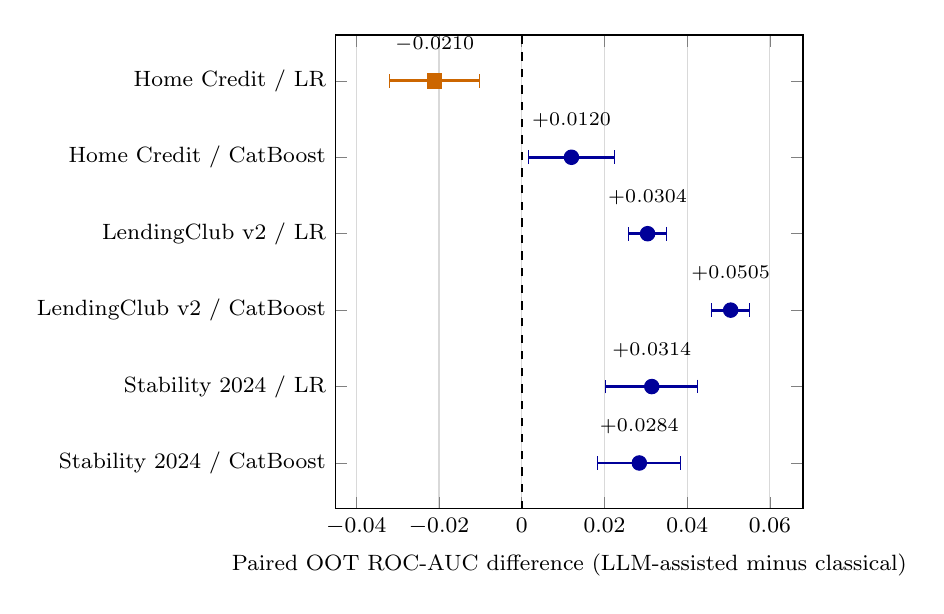
\begin{tikzpicture}
\begin{axis}[
    width=0.62\linewidth, height=7.6cm,
    xlabel={Paired OOT ROC-AUC difference (LLM-assisted minus classical)},
    xmin=-0.045, xmax=0.068,
    scaled x ticks=false,
    xtick={-0.04,-0.02,0,0.02,0.04,0.06},
    xticklabel style={/pgf/number format/fixed, /pgf/number format/precision=2},
    ytick={1,2,3,4,5,6},
    yticklabels={Stability 2024 / CatBoost, Stability 2024 / LR, LendingClub v2 / CatBoost, LendingClub v2 / LR, Home Credit / CatBoost, Home Credit / LR},
    ymin=0.4, ymax=6.6,
    xmajorgrids, grid style={gray!30},
    tick label style={font=\footnotesize}, label style={font=\footnotesize},
    clip=false,
]
\draw[black, thick, dashed] (axis cs:0,0.4) -- (axis cs:0,6.6);
\addplot[only marks, mark=*, mark size=2.6pt, blue!60!black,
    error bars/.cd, x dir=both, x explicit,
    error bar style={line width=1pt, blue!60!black},
    error mark options={rotate=90, mark size=2.5pt, blue!60!black}]
    coordinates {
        (0.028431,1) +- (0.010022,0)
        (0.031444,2) +- (0.011125,0)
        (0.050517,3) +- (0.004558,0)
        (0.030431,4) +- (0.004665,0)
        (0.012024,5) +- (0.010492,0)
    };
\addplot[only marks, mark=square*, mark size=2.6pt, orange!80!black,
    error bars/.cd, x dir=both, x explicit,
    error bar style={line width=1pt, orange!80!black},
    error mark options={rotate=90, mark size=2.5pt, orange!80!black}]
    coordinates { (-0.021033,6) +- (0.010874,0) };
\node[font=\scriptsize, above=7pt] at (axis cs:0.028431,1) {$+0.0284$};
\node[font=\scriptsize, above=7pt] at (axis cs:0.031444,2) {$+0.0314$};
\node[font=\scriptsize, above=7pt] at (axis cs:0.050517,3) {$+0.0505$};
\node[font=\scriptsize, above=7pt] at (axis cs:0.030431,4) {$+0.0304$};
\node[font=\scriptsize, above=7pt] at (axis cs:0.012024,5) {$+0.0120$};
\node[font=\scriptsize, above=7pt] at (axis cs:-0.021033,6) {$-0.0210$};
\end{axis}
\end{tikzpicture}
\caption{Paired locked-OOT ROC-AUC differences between the best LLM-assisted and the best classical selector in each dataset--backbone case, with 95\% confidence intervals. Positive values favour LLM-assisted selection; the square marks the one case in which the classical selector (mRMR) is significantly higher.}
\label{fig:paired_auc}
\end{figure}

The pattern is dataset- and model-specific rather than uniform. LendingClub v2 and Stability 2024 favour LLM-assisted selection under both backbones: pure LLM screening is the best LLM-assisted selector in three of those four cases and LLM then mRMR in the fourth, and the differences are moderate to large in the reporting bands of Section~\ref{subsec:inference}, from $+0.028$ to $+0.051$. Home Credit is mixed. With CatBoost, pure LLM screening exceeds the RFE CatBoost wrapper by $+0.012$; with logistic regression, mutual-information mRMR exceeds the best LLM-assisted pipeline, stable core plus LLM fill, by $0.021$. The best classical comparator differs by case: mRMR for Home Credit logistic regression, RFE CatBoost for both CatBoost cases on Home Credit and Stability, and IV then Boruta for both LendingClub cases and Stability logistic regression. The largest gain occurs on LendingClub with CatBoost; LendingClub is the dataset whose eligible universe after screening is the smallest (161 of 675 features) and whose OOT event rate is the highest.

\begin{table}[htbp]
\centering
\scriptsize
\begin{threeparttable}
\caption{Full-feature reference models compared with the best selected subset in each case. Differences are descriptive point estimates; no paired interval is computed against the full-feature reference.}
\label{tab:full_feature}
\begin{tabular}{@{}llrlrr@{}}
\toprule
Dataset & Model & Full AUC & Best subset & Subset AUC & Subset $-$ full \\
\midrule
Home Credit & LR & 0.771496 & mRMR & 0.769890 & $-0.001606$ \\
Home Credit & CatBoost & 0.786032 & Pure LLM & 0.793450 & $+0.007418$ \\
LendingClub v2 & LR & 0.710887 & Pure LLM & 0.740234 & $+0.029347$ \\
LendingClub v2 & CatBoost & 0.722973 & LLM then mRMR & 0.770664 & $+0.047691$ \\
Stability 2024 & LR & 0.7734 & Pure LLM & 0.834400 & $+0.0610$ \\
Stability 2024 & CatBoost & 0.8105 & Pure LLM & 0.878400 & $+0.0679$ \\
\bottomrule
\end{tabular}
\end{threeparttable}
\end{table}

Table~\ref{tab:full_feature} and Figure~\ref{fig:selector_auc} place the selected subsets against models fitted on the full eligible feature universe. In five of six cases the best compact subset of 20 or 40 original features has a higher OOT AUC than the full-feature model, by margins that range from $+0.007$ (Home Credit CatBoost) to $+0.068$ (Stability 2024 CatBoost); the exception is again Home Credit logistic regression, where the full-feature model is $0.0016$ above the mRMR subset. Compact selection therefore does not cost discrimination on these portfolios, and on LendingClub and Stability it improves it substantially, which is consistent with redundancy and noise in the wide engineered universes degrading both the regularised linear model and the boosted model out of time.

\begin{figure}[htbp]
\centering
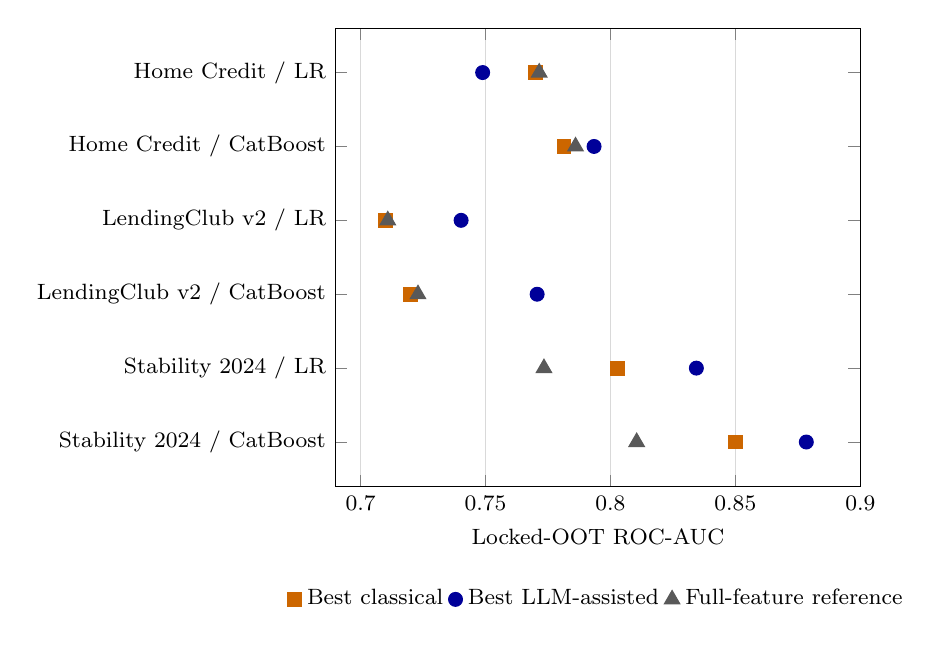
\begin{tikzpicture}
\begin{axis}[
    width=0.68\linewidth, height=7.4cm,
    xlabel={Locked-OOT ROC-AUC},
    xmin=0.69, xmax=0.90,
    ytick={1,2,3,4,5,6},
    yticklabels={Stability 2024 / CatBoost, Stability 2024 / LR, LendingClub v2 / CatBoost, LendingClub v2 / LR, Home Credit / CatBoost, Home Credit / LR},
    ymin=0.4, ymax=6.6,
    xmajorgrids, grid style={gray!30},
    tick label style={font=\footnotesize}, label style={font=\footnotesize},
    legend style={at={(0.5,-0.2)}, anchor=north, legend columns=3, font=\footnotesize, draw=none},
]
\addplot[only marks, mark=square*, mark size=2.5pt, orange!80!black]
    coordinates {(0.849969,1) (0.802956,2) (0.720147,3) (0.709803,4) (0.781426,5) (0.769890,6)};
\addlegendentry{Best classical}
\addplot[only marks, mark=*, mark size=2.5pt, blue!60!black]
    coordinates {(0.878400,1) (0.834400,2) (0.770664,3) (0.740234,4) (0.793450,5) (0.748857,6)};
\addlegendentry{Best LLM-assisted}
\addplot[only marks, mark=triangle*, mark size=3.2pt, gray!70!black]
    coordinates {(0.8105,1) (0.7734,2) (0.722973,3) (0.710887,4) (0.786032,5) (0.771496,6)};
\addlegendentry{Full-feature reference}
\end{axis}
\end{tikzpicture}
\caption{Locked-OOT ROC-AUC of the best classical selector, the best LLM-assisted selector and the full-feature reference model in each dataset--backbone case. Comparisons are meaningful within a row; absolute levels differ across datasets because event rates, feature universes and time windows differ.}
\label{fig:selector_auc}
\end{figure}

\subsection{Secondary Metrics}
\label{subsec:secondary_results}

Secondary metrics are reported as the best value attained by any selector in each dataset, together with the identity of the selector and backbone that attained it (Table~\ref{tab:secondary}). Because the leading selector differs from metric to metric, these values describe the frontier reached by the selector family in each dataset rather than a single model, and they must not be combined into one scorecard. The full grid of fifteen metric families is given in Appendix~\ref{app:supplementary}.

\begin{table}[htbp]
\centering
\footnotesize
\begin{threeparttable}
\caption{Best locked-OOT secondary metrics by dataset, with the selector and backbone attaining each value. KS is the maximum separation over OOT thresholds; Brier is lower-is-better; Capture@10 is the share of events in the highest-scored decile.}
\label{tab:secondary}
\begin{tabular}{@{}lllll@{}}
\toprule
Dataset & Metric & Best value & Selector & Backbone \\
\midrule
Home Credit & KS & 0.450543 & Pure LLM & CatBoost \\
Home Credit & Brier score & 0.153354 & Pure LLM & CatBoost \\
Home Credit & Capture@10 & 0.358065 & RFE CatBoost & CatBoost \\
LendingClub v2 & KS & 0.394310 & LLM then mRMR & CatBoost \\
LendingClub v2 & Brier score & 0.202423 & LLM then mRMR & CatBoost \\
LendingClub v2 & Capture@10 & 0.226851 & IV then Boruta & CatBoost \\
Stability 2024 & KS & 0.593430 & LLM then mRMR & CatBoost \\
Stability 2024 & Brier score & 0.179236 & Pure LLM & CatBoost \\
Stability 2024 & Capture@10 & 0.507606 & RFE CatBoost & CatBoost \\
\bottomrule
\end{tabular}
\end{threeparttable}
\end{table}

\paragraph{Separation and probability quality}
The best KS is attained by an LLM-assisted CatBoost pipeline in all three datasets: pure LLM on Home Credit and LLM then mRMR on LendingClub and Stability. The best Brier score is likewise attained by the LLM-assisted CatBoost pipelines that lead AUC (pure LLM on Home Credit and Stability, LLM then mRMR on LendingClub), and the corresponding log losses of those three CatBoost models are 0.469725, 0.589022 and 0.532077. Reliability curves of the AUC-winning CatBoost models over ten equal-frequency probability bins track the diagonal without systematic reversal, but because both backbones are fitted with balanced class weights their probabilities are shifted away from the natural event rate, so Brier and log loss are used only to compare selectors within a dataset and not as absolute calibration claims (Section~\ref{subsec:limitations}).

\paragraph{Top-decile concentration}
The highest-scored decile captures between 22.7\% and 50.8\% of events depending on the portfolio, corresponding to Lift@10 values of 3.58 (Home Credit), 2.27 (LendingClub) and 5.08 (Stability 2024). The leading selector for concentration is a classical wrapper in every dataset: RFE CatBoost on Home Credit and Stability, and IV then Boruta on LendingClub. Concentration and discrimination therefore have different leaders, which is expected because Capture@10 summarises only the upper tail of the score distribution.

\paragraph{Temporal stability}
Score PSI between DEV and OOT is small for every leading pipeline. The lowest score PSI in each dataset is 0.000873 (Home Credit, LLM then Boruta with logistic regression), 0.000599 (LendingClub, Random K with CatBoost) and 0.000210 (Stability, LLM then mRMR with CatBoost), all far below the 0.10 monitoring reference. Selected-feature PSI is likewise small: the lowest mean feature PSI is 0.001365 on Home Credit (Boruta RF), 0.000057 on LendingClub (domain rules) and 0.006800 on Stability (LLM then mRMR, logistic regression), and the lowest maximum feature PSI is 0.011861, 0.001113 and 0.093000 respectively. Stability 2024 has the largest maximum selected-feature drift, reflecting its longer and calendar-anchored OOT window, while its score PSI remains the lowest of the three datasets. Median selected-feature PSI is zero for the pure LLM subsets on Home Credit under both backbones, so the typical semantically selected variable did not shift measurably between development and OOT.

\subsection{Feature-Selection Stability}
\label{subsec:stability_results}

Table~\ref{tab:classical_stability} reports the most reproducible independently refitted selector in each dataset--backbone case, ordered by Nogueira stability with mean pairwise Jaccard as tie-breaker. Boruta RF on LendingClub logistic regression is the most reproducible selector in the study, with Nogueira stability 0.9588 and Jaccard 0.9273; IV/WOE leads four of the six cases, and mRMR leads LendingClub CatBoost. Stability is lower on Stability 2024, where the candidate universe is far larger (1,959 features), with Nogueira values near 0.78 and Jaccard near 0.66. These values quantify fold-to-fold agreement of the target-aware selectors; the pure LLM subset is a fixed ranking reused across folds and is therefore excluded from this comparison, and the hybrids inherit the reproducibility of their statistical stage.

\begin{table}[htbp]
\centering
\footnotesize
\begin{threeparttable}
\caption{Most reproducible independently refitted selector in each case across the five development folds (Nogueira stability as the primary ordering, mean pairwise Jaccard as tie-breaker).}
\label{tab:classical_stability}
\begin{tabular}{@{}llllrr@{}}
\toprule
Dataset & Model & Selector & $\Kfeat$ & Nogueira & Jaccard \\
\midrule
Home Credit & LR & IV/WOE & 20 & 0.8857 & 0.8053 \\
Home Credit & CatBoost & IV/WOE & 40 & 0.8458 & 0.7538 \\
LendingClub v2 & LR & Boruta RF & 20 & 0.9588 & 0.9273 \\
LendingClub v2 & CatBoost & mRMR & 40 & 0.9070 & 0.8462 \\
Stability 2024 & LR & IV/WOE & 20 & 0.7878 & 0.6666 \\
Stability 2024 & CatBoost & IV/WOE & 40 & 0.7831 & 0.6582 \\
\bottomrule
\end{tabular}
\end{threeparttable}
\end{table}

The reproducibility of the contrastive branch is the primary outcome of the CLIP extension and is reported in Table~\ref{tab:clip_stability} and Figure~\ref{fig:clip_stability}. All six source--backbone cells that rank Stability 2024 features achieve Nogueira stability between 0.683 and 0.753 and Jaccard between 0.657 and 0.723 across the five folds. The Home Credit source representation with logistic regression is the most reproducible cell on both measures (0.7525 and 0.7225), followed by the native Stability representation with logistic regression on Nogueira (0.7225) and the LendingClub representation with CatBoost on Jaccard (0.7175). The CLIP-ranked cells are therefore close to the classical stability leaders on the same dataset (0.7878 and 0.7831), even though their downstream redundancy stage starts from a much smaller pool of 60 or 100 candidates.

\begin{table}[htbp]
\centering
\footnotesize
\begin{threeparttable}
\caption{Fold-to-fold reproducibility of CLIP-ranked selection on Stability 2024, by source representation and backbone. $P$ is the candidate pool passed to legacy RF/correlation mRMR and $\Kfeat$ the retained budget.}
\label{tab:clip_stability}
\begin{tabular}{@{}llrrrr@{}}
\toprule
Source $\rightarrow$ target & Model & $P$ & $\Kfeat$ & Nogueira & Jaccard \\
\midrule
Stability $\rightarrow$ Stability & LR & 60 & 20 & 0.722500 & 0.697266 \\
Stability $\rightarrow$ Stability & CatBoost & 100 & 40 & 0.683333 & 0.688861 \\
Home Credit $\rightarrow$ Stability & LR & 60 & 20 & 0.752500 & 0.722518 \\
Home Credit $\rightarrow$ Stability & CatBoost & 100 & 40 & 0.712500 & 0.710146 \\
LendingClub $\rightarrow$ Stability & LR & 60 & 20 & 0.685000 & 0.656678 \\
LendingClub $\rightarrow$ Stability & CatBoost & 100 & 40 & 0.720833 & 0.717478 \\
\bottomrule
\end{tabular}
\end{threeparttable}
\end{table}

\begin{figure}[htbp]
\centering
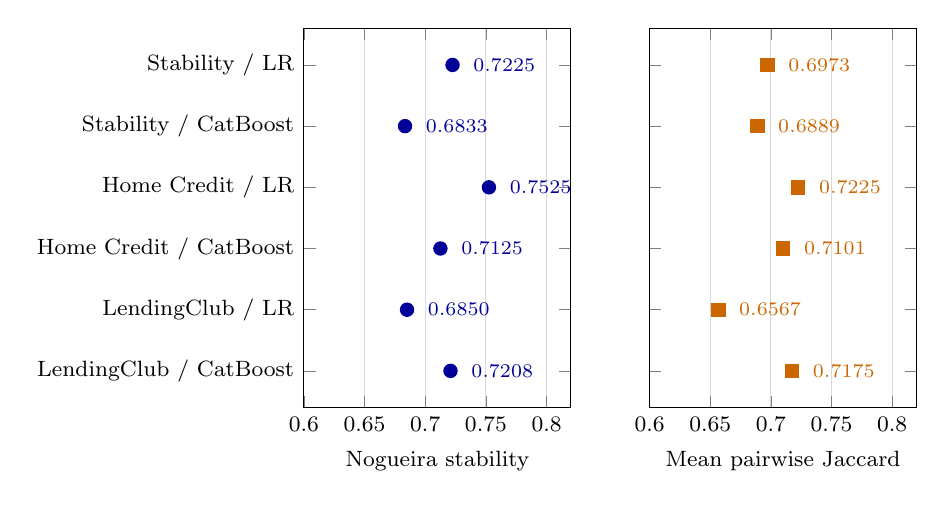
\begin{tikzpicture}
\begin{groupplot}[
    group style={group size=2 by 1, horizontal sep=10mm, y descriptions at=edge left},
    width=0.41\linewidth, height=6.4cm,
    ytick={1,2,3,4,5,6},
    yticklabels={LendingClub / CatBoost, LendingClub / LR, Home Credit / CatBoost, Home Credit / LR, Stability / CatBoost, Stability / LR},
    ymin=0.4, ymax=6.6, xmin=0.60, xmax=0.82,
    xmajorgrids, grid style={gray!30},
    tick label style={font=\footnotesize}, label style={font=\footnotesize},
    nodes near coords={\pgfmathprintnumber[fixed,precision=4,zerofill]{\pgfplotspointmeta}},
    nodes near coords style={font=\scriptsize, anchor=west, xshift=4pt},
    point meta=x,
]
\nextgroupplot[xlabel={Nogueira stability}]
\addplot[only marks, mark=*, mark size=2.4pt, blue!60!black]
    coordinates {(0.720833,1) (0.685000,2) (0.712500,3) (0.752500,4) (0.683333,5) (0.722500,6)};
\nextgroupplot[xlabel={Mean pairwise Jaccard}]
\addplot[only marks, mark=square*, mark size=2.4pt, orange!80!black]
    coordinates {(0.717478,1) (0.656678,2) (0.710146,3) (0.722518,4) (0.688861,5) (0.697266,6)};
\end{groupplot}
\end{tikzpicture}
\caption{Fold-to-fold reproducibility of CLIP-ranked subsets on Stability 2024 for the three source representations and two backbones. Higher is more reproducible.}
\label{fig:clip_stability}
\end{figure}

\subsection{CLIP Results}
\label{subsec:clip_results}

\paragraph{Downstream performance}
Table~\ref{tab:clip_performance} and Figure~\ref{fig:clip_performance} report the locked-OOT performance of the six CLIP-ranked cells on the contrastive extension cohort of Stability 2024 (304,916 decisions, 8,349 events). Within the extension, the native Stability representation with CatBoost has the highest OOT AUC (0.772872), followed by the Home Credit source (0.761999) and the LendingClub source (0.750327); CatBoost exceeds logistic regression under every source. For logistic regression the ordering differs: the Home Credit source ranking (0.7064) is 0.0287 above the native ranking (0.6777) and the LendingClub source (0.6679) is 0.0099 below it. These values describe the complete pipeline of contrastive ranking, target-aware legacy mRMR and a target-trained classifier; they are not retrieval metrics of the representation itself, and they are below the AUC of the pure LLM and classical selectors on the headline Stability cohort (Table~\ref{tab:primary_results}), which is why the contrastive branch is evaluated primarily on reproducibility and portability rather than on maximum discrimination.

\begin{table}[htbp]
\centering
\scriptsize
\setlength{\tabcolsep}{4pt}
\begin{threeparttable}
\caption{Locked-OOT performance of CLIP-ranked subsets on the Stability 2024 extension cohort (OOT from 2020-02-26; $N=304{,}916$; 8,349 events), by source representation and backbone. Logistic regression uses pool 60 and $\Kfeat=20$; CatBoost uses pool 100 and $\Kfeat=40$. KS, Lift@10 and Capture@10 are reported at the precision of the study's figures; the last column is OOT AUC minus pooled DEV out-of-fold AUC.}
\label{tab:clip_performance}
\begin{tabular}{@{}llrrrrr@{}}
\toprule
Source representation & Model & OOT AUC & OOT KS & Lift@10 & Capture@10 & OOT $-$ DEV OOF \\
\midrule
Stability 2024 & LR & 0.6777 & 0.269 & 2.67 & 0.267 & $+0.0210$ \\
Stability 2024 & CatBoost & 0.772872 & 0.412 & 3.71 & 0.371 & $+0.0169$ \\
Home Credit & LR & 0.7064 & 0.309 & 2.81 & 0.281 & $+0.0336$ \\
Home Credit & CatBoost & 0.761999 & 0.388 & 3.55 & 0.355 & $+0.0161$ \\
LendingClub v2 & LR & 0.6679 & 0.240 & 2.51 & 0.251 & $+0.0452$ \\
LendingClub v2 & CatBoost & 0.750327 & 0.372 & 3.59 & 0.359 & $+0.0246$ \\
\bottomrule
\end{tabular}
\end{threeparttable}
\end{table}

\begin{figure}[htbp]
\centering
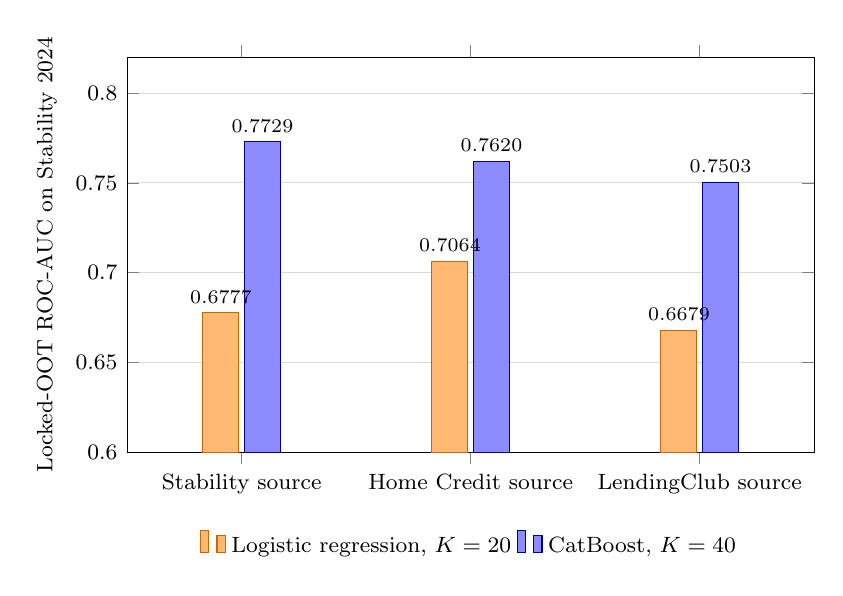
\begin{tikzpicture}
\begin{axis}[
    ybar, bar width=13pt,
    width=0.85\linewidth, height=6.6cm,
    ymin=0.60, ymax=0.82,
    ylabel={Locked-OOT ROC-AUC on Stability 2024},
    symbolic x coords={Stability source, Home Credit source, LendingClub source},
    xtick=data, enlarge x limits=0.25,
    ymajorgrids, grid style={gray!30},
    legend style={at={(0.5,-0.18)}, anchor=north, legend columns=2, font=\footnotesize, draw=none},
    nodes near coords, nodes near coords style={font=\scriptsize, /pgf/number format/.cd, fixed, precision=4, zerofill},
    tick label style={font=\footnotesize}, label style={font=\footnotesize},
]
\addplot[fill=orange!55, draw=orange!80!black]
    coordinates {(Stability source,0.6777) (Home Credit source,0.7064) (LendingClub source,0.6679)};
\addlegendentry{Logistic regression, $\Kfeat=20$}
\addplot[fill=blue!45, draw=blue!60!black]
    coordinates {(Stability source,0.772872) (Home Credit source,0.761999) (LendingClub source,0.750327)};
\addlegendentry{CatBoost, $\Kfeat=40$}
\end{axis}
\end{tikzpicture}
\caption{Locked-OOT ROC-AUC of CLIP-ranked subsets on the Stability 2024 extension cohort for the three source representations. Transferred rankings from Home Credit and LendingClub are applied to Stability features without refitting.}
\label{fig:clip_performance}
\end{figure}

\paragraph{DEV-to-OOT generalisation}
All six OOT AUC values lie above the corresponding pooled DEV out-of-fold AUC, by $+0.016$ to $+0.045$ (last column of Table~\ref{tab:clip_performance}). The CLIP-ranked subsets therefore do not collapse when the temporal holdout is opened; the improvement on OOT reflects the difference between the fold-validation populations and the later cohort rather than optimism, since the representation stage consumed no OOT information and the redundancy stage and classifiers were fitted on fold training partitions.

\paragraph{Representation diagnostics}
Table~\ref{tab:clip_seeds} reports the five seed checkpoints of the native Stability representation. Validation mean reciprocal rank ranges from 0.2255 to 0.2651 over 395 held-out feature pairs, Recall@10 from 0.472 to 0.546, and the margin between positive-pair and allowed-negative cosine similarity from 0.528 to 0.568, so every seed learned a cross-view alignment well above chance and no single seed dominates. All twenty collapse diagnostics passed. These are alignment diagnostics of the representation, distinct from the fold-level subset stability of Table~\ref{tab:clip_stability}.

\begin{table}[htbp]
\centering
\scriptsize
\begin{threeparttable}
\caption{Five-seed checkpoint diagnostics of the native Stability 2024 contrastive representation. Checkpoints are selected by minimum source-validation loss; retrieval metrics are computed on 395 validation feature pairs.}
\label{tab:clip_seeds}
\begin{tabular}{@{}rrrrrrrr@{}}
\toprule
Seed & Best epoch & Validation loss & MRR & Recall@1 & Recall@5 & Recall@10 & Cosine margin \\
\midrule
11 & 37 & 4.096998 & 0.2255 & 0.100 & 0.347 & 0.510 & 0.528 \\
22 & 60 & 4.063112 & 0.2587 & 0.132 & 0.396 & 0.538 & 0.555 \\
33 & 70 & 4.053390 & 0.2635 & 0.142 & 0.387 & 0.542 & 0.544 \\
44 & 69 & 4.103792 & 0.2651 & 0.141 & 0.405 & 0.546 & 0.568 \\
55 & 46 & 4.094028 & 0.2466 & 0.129 & 0.358 & 0.472 & 0.535 \\
\bottomrule
\end{tabular}
\end{threeparttable}
\end{table}

\paragraph{Cross-source ranking agreement and transfer}
The three source representations do not produce one universal ordering of the Stability predictors (Table~\ref{tab:clip_agreement}). The native Stability ranking and the Home Credit ranking share only 6 of their top 100 features (Spearman $\rho=0.264$ over all 1,959 features); Stability and LendingClub share 45 ($\rho=0.426$); Home Credit and LendingClub share a single feature ($\rho=0.004$). Transfer is therefore source-dependent. Compared with the earlier experiments in which the same source representations ranked Home Credit features, the Home Credit source with CatBoost is almost unchanged when applied to Stability (0.7627 on Home Credit against 0.7620 on Stability), the Home Credit source with logistic regression falls by 0.0272, and the LendingClub source improves markedly on the new target (from 0.6766 to 0.7503 with CatBoost and from 0.5732 to 0.6679 with logistic regression). Because each source carries its own descriptor transform, projection geometry and anchor, the same Stability features are scored through different learned coordinate systems, and the target-aware redundancy stage followed by a target-trained classifier recovers part of the useful signal even when the transferred ranking differs strongly from the native one. Score PSI of the CLIP-ranked cells is below 0.10 in five of six cells; the Home Credit source with CatBoost shows moderate score drift (0.153625).

\begin{table}[htbp]
\centering
\footnotesize
\begin{threeparttable}
\caption{Agreement between the three source-specific rankings of the 1,959 Stability 2024 features. Spearman correlation is computed over all features; the last column counts features shared by the two top-100 lists.}
\label{tab:clip_agreement}
\begin{tabular}{@{}llrr@{}}
\toprule
Source A & Source B & Spearman $\rho$ & Shared top-100 features \\
\midrule
Stability 2024 & Home Credit & 0.264 & 6 \\
Stability 2024 & LendingClub v2 & 0.426 & 45 \\
Home Credit & LendingClub v2 & 0.004 & 1 \\
\bottomrule
\end{tabular}
\end{threeparttable}
\end{table}

\paragraph{Incremental value after LLM screening}
The reason the contrastive branch is assessed on reproducibility is visible in its original Home Credit evaluation (Appendix~\ref{app:development}, Table~\ref{tab:clip_increment}). Inserting the corrected contrastive ranking between LLM screening and mRMR changed OOT AUC by $-0.001102$ for logistic regression and $+0.000866$ for CatBoost, while mean pairwise Jaccard of the selected subsets rose by $+0.324841$ and $+0.498638$ and CatBoost score PSI fell from 0.008286 to 0.004094. The representation imposes a coherent ordering inside the semantically screened pool, which makes fold-selected subsets far more reproducible, but the pool already contains the strong predictors, so discrimination is essentially unchanged.

\subsection{Voting Results}
\label{subsec:voting_results}

Table~\ref{tab:voting} and Figure~\ref{fig:voting} report the eight Home Credit voting variants against two references: the sequential pipeline LLM then mRMR that they are designed to improve on, and the full-pool mRMR selector applied to all 529 features. Voting exceeds the sequential comparator in five of eight comparisons and never exceeds the full-pool reference. Among the pool-based variants, AUC increases monotonically with the pool size $P$ for both backbones: from 0.739432 at $P=100$ to 0.744653 at $P=300$ for logistic regression, and from 0.758757 to 0.766448 for CatBoost. Against the sequential comparator, the logistic-regression gains at $P=200$ and $P=300$ ($+0.0059$ and $+0.0066$) and the CatBoost gain at $P=300$ ($+0.0035$) are Holm-significant within the 24-test voting family; the $P=100$ CatBoost variant and the direct three-voter CatBoost variant are significantly below the sequential comparator. The direct three-voter selector, which averages the LLM, contrastive and mRMR relevance ranks and selects $\Kfeat$ without a refinement stage, is weaker than the best pool-based variant under both backbones. The CatBoost $P=300$ variant comes within 0.000391 of the full-pool mRMR reference (0.766448 against 0.766839), so parallel aggregation of the semantic and contrastive rankings recovers almost all the information that sequential screening discarded, but it does not surpass statistical selection from the complete universe.

\begin{sidewaystable}[htbp]
\centering
\scriptsize
\begin{threeparttable}
\caption{Home Credit voting experiment. The sequential comparator is LLM then mRMR; the full-pool reference is mRMR on all 529 features. $\Delta$ is voting minus sequential; $p$-values are Holm-adjusted within the family of 24 voting tests.}
\label{tab:voting}
\begin{tabular}{@{}llrrrlr@{}}
\toprule
Model & Variant & Voting AUC & Sequential AUC & $\Delta$ vs sequential & Holm $p$ & Full-pool mRMR AUC \\
\midrule
LR & LLM+CLIP, $P=100$, then mRMR & 0.739432 & 0.738098 & $+0.001334$ & 0.3862 & 0.769890 \\
LR & LLM+CLIP, $P=200$, then mRMR & 0.744020 & 0.738098 & $+0.005921$ & $3.7\times10^{-8}$ & 0.769890 \\
LR & LLM+CLIP, $P=300$, then mRMR & 0.744653 & 0.738098 & $+0.006554$ & $1.7\times10^{-10}$ & 0.769890 \\
LR & Direct three-voter, $\Kfeat=20$ & 0.740573 & 0.738098 & $+0.002474$ & 0.1217 & 0.769890 \\
CatBoost & LLM+CLIP, $P=100$, then mRMR & 0.758757 & 0.762954 & $-0.004197$ & 0.0408 & 0.766839 \\
CatBoost & LLM+CLIP, $P=200$, then mRMR & 0.759263 & 0.762954 & $-0.003691$ & 0.0638 & 0.766839 \\
CatBoost & LLM+CLIP, $P=300$, then mRMR & 0.766448 & 0.762954 & $+0.003495$ & 0.0422 & 0.766839 \\
CatBoost & Direct three-voter, $\Kfeat=40$ & 0.754521 & 0.762954 & $-0.008433$ & $5.7\times10^{-7}$ & 0.766839 \\
\bottomrule
\end{tabular}
\end{threeparttable}
\end{sidewaystable}

\begin{figure}[htbp]
\centering
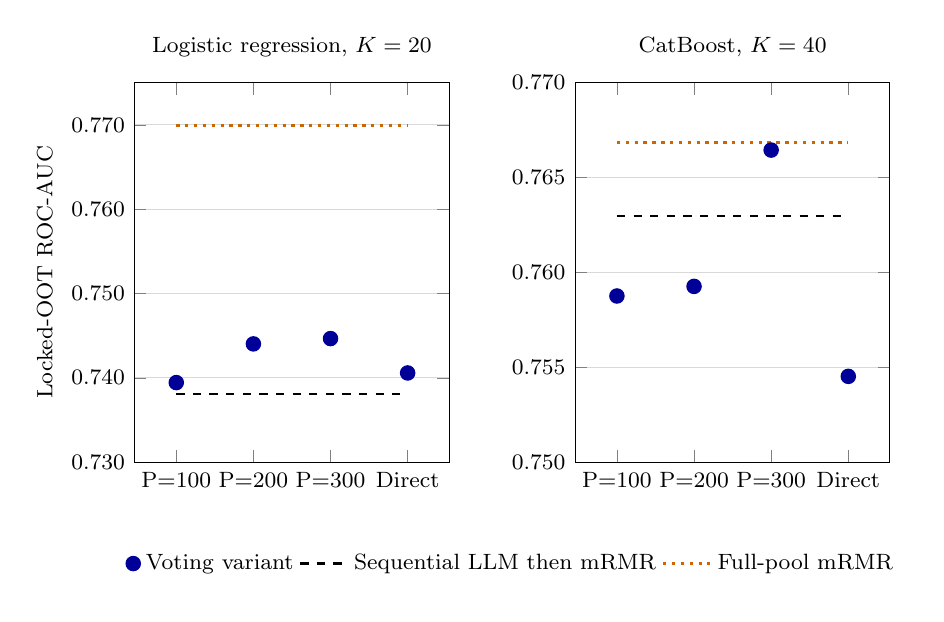
\begin{tikzpicture}
\begin{groupplot}[
    group style={group size=2 by 1, horizontal sep=16mm},
    width=0.46\linewidth, height=6.4cm,
    symbolic x coords={P=100,P=200,P=300,Direct},
    xtick=data, enlarge x limits=0.18,
    ymajorgrids, grid style={gray!30},
    yticklabel style={/pgf/number format/fixed, /pgf/number format/precision=3, /pgf/number format/zerofill},
    tick label style={font=\footnotesize}, label style={font=\footnotesize},
    legend style={font=\footnotesize, draw=none},
]
\nextgroupplot[title={Logistic regression, $\Kfeat=20$}, title style={font=\footnotesize}, ylabel={Locked-OOT ROC-AUC}, ymin=0.730, ymax=0.775, ytick distance=0.010,
    legend to name=votinglegend, legend columns=3]
\addplot[only marks, mark=*, mark size=2.6pt, blue!60!black] coordinates {(P=100,0.739432) (P=200,0.744020) (P=300,0.744653) (Direct,0.740573)};
\addlegendentry{Voting variant}
\addplot[dashed, thick, black] coordinates {(P=100,0.738098) (Direct,0.738098)};
\addlegendentry{Sequential LLM then mRMR}
\addplot[dotted, very thick, orange!80!black] coordinates {(P=100,0.769890) (Direct,0.769890)};
\addlegendentry{Full-pool mRMR}
\nextgroupplot[title={CatBoost, $\Kfeat=40$}, title style={font=\footnotesize}, ymin=0.750, ymax=0.770, ytick distance=0.005]
\addplot[only marks, mark=*, mark size=2.6pt, blue!60!black] coordinates {(P=100,0.758757) (P=200,0.759263) (P=300,0.766448) (Direct,0.754521)};
\addplot[dashed, thick, black] coordinates {(P=100,0.762954) (Direct,0.762954)};
\addplot[dotted, very thick, orange!80!black] coordinates {(P=100,0.766839) (Direct,0.766839)};
\end{groupplot}
\node[anchor=north] at ($(group c1r1.south)!0.5!(group c2r1.south) + (0,-9mm)$) {\pgfplotslegendfromname{votinglegend}};
\end{tikzpicture}
\caption{Home Credit voting AUC by candidate-pool size, with the sequential comparator (LLM then mRMR) and the full-pool mRMR reference for each backbone. The vertical scales differ between panels.}
\label{fig:voting}
\end{figure}

\subsection{Operational Cost of the LLM Stage}
\label{subsec:cost_results}

The semantic stage is inexpensive relative to model fitting. In the development experiments on Home Credit and LendingClub, the 72 canonical logical screening requests were served by 30 physical provider calls, of which 24 were canonical ranking calls and 6 generated source descriptions; 48 requests were answered from the local cache. Provider-reported usage was 806,757 input tokens and 56,495 output tokens, and because cached-input billing shares were not retained the direct API cost is bounded between USD~0.171 and USD~0.413 at the rates in force; without reuse the same requests would have cost between USD~0.625 and USD~1.396. In the same experiments the pure LLM pipeline for Home Credit logistic regression completed in 0.8 minutes against 12.1 minutes for full-pool mRMR, although runtime comparisons were made under unequal caching and execution conditions and are descriptive only. Extrapolated scenarios for a 2,000-feature universe are given in Appendix~\ref{app:supplementary}. The cost of the final three-dataset experiment was not separately metered.

% ============================================================
% 7. DISCUSSION
% ============================================================

\section{Discussion}
\label{sec:discussion}

\subsection{Main Findings}
\label{subsec:main_findings}

The first research question asked whether an LLM-screened subset can match or exceed classically selected subsets out of time under a fixed budget. The answer is affirmative but conditional. In five of six dataset--backbone cases the best LLM-assisted selector attains a significantly higher locked-OOT ROC-AUC than the best classical selector, and in five of six cases the best compact subset also exceeds the full-feature model. The exception, Home Credit logistic regression, is not a marginal case: mutual-information mRMR exceeds the best LLM-assisted pipeline by 0.021, a large difference in the reporting bands, and the full-feature model is marginally above both. Semantic screening is therefore a strong first-pass filter whose benefit depends on the portfolio and on the downstream model; it is not a universal replacement for statistical selection.

The second question concerned reproducibility. Independently refitted classical selectors reach Nogueira stability between 0.78 and 0.96 across the six cases, with information value and Boruta the most reproducible. The contrastive ranking followed by legacy mRMR reaches 0.68 to 0.75 on the largest universe, close to the classical leaders there, and its original Home Credit evaluation showed that inserting the representation into an LLM-screened pipeline raised fold-to-fold Jaccard similarity by 0.32 to 0.50 while leaving discrimination essentially unchanged. Reproducibility and discrimination are thus separable outcomes: the representation improves the former without buying or costing the latter.

The third question concerned portability. Representations trained on three portfolios rank the same Stability predictors very differently (shared top-100 counts of 6, 45 and 1), yet every transferred ranking still supports a downstream model whose OOT AUC exceeds its development estimate, and the LendingClub source, which was weak when transferred to Home Credit, is competitive when transferred to Stability. Portability is therefore real but source-dependent, and the target-aware redundancy stage and target-trained classifier recover much of the signal that a mismatched ranking loses.

The fourth question concerned the order of combination. Parallel rank voting recovers information discarded by sequential screening in five of eight Home Credit comparisons, with three Holm-significant gains, and its AUC rises monotonically with pool size, but no voting variant exceeds mRMR applied to the full universe. The practical reading is that when a strong statistical selector can be run on the complete universe, the ordering of semantic and statistical stages matters less than giving the statistical stage a sufficiently large pool.

\subsection{Predictive Performance vs Stability}
\label{subsec:performance_vs_stability}

The results show three trade-offs. First, the LLM-assisted pipelines that lead discrimination on LendingClub and Stability are built on a fixed cached ranking, so their fold agreement is perfect by construction and uninformative; their reproducibility as deployed selectors depends on the reproducibility of the language model itself under a fixed snapshot and prompt, which the study controls by caching rather than by repeated calls. Second, the classical selectors that lead reproducibility (IV/WOE, Boruta RF) are not the ones that lead discrimination in most cases, and the classical selectors that are most competitive on AUC (RFE CatBoost, IV then Boruta, mRMR) are wrappers or greedy procedures that are more sensitive to the training sample. Third, the contrastive representation and the stable-core construction are the two devices in the study that raise reproducibility of a semantically screened subset without a systematic loss of discrimination; the stable-core hybrid is also the best LLM-assisted pipeline on Home Credit logistic regression, although it remains below mRMR there.

Subset size interacts with these trade-offs. The larger CatBoost budget benefits every family, and the boosted model is less sensitive to redundant predictors, which is consistent with the decision to fix $\Kfeat=40$ for CatBoost and $\Kfeat=20$ for logistic regression. Temporal behaviour is favourable throughout: score PSI of every leading pipeline is far below the conventional 0.10 reference, and the semantically selected subsets show the smallest median feature drift on Home Credit. Whether lower feature drift translates into lower score drift or better discrimination is not established by these data; the two quantities move independently across selectors.

\subsection{Cross-Dataset Behavior}
\label{subsec:cross_dataset}

Several findings reproduce across datasets and backbones. The best compact subset exceeds the full-feature model in every case except Home Credit logistic regression. CatBoost exceeds logistic regression in every headline case, for every full-feature reference and in every CLIP-ranked cell. An LLM-assisted CatBoost pipeline attains the best KS and the best Brier score in all three datasets, and a classical wrapper attains the best top-decile concentration in all three. Score drift is negligible everywhere.

Other findings are dataset- or model-specific. The direction of the headline comparison reverses between Home Credit logistic regression and the other five cases. The best classical comparator changes identity across cases, so a single classical baseline would have misrepresented the strength of classical selection. The magnitude of the LLM-assisted gain is largest on LendingClub, where eligibility screening removes most of the universe and the resolved-outcome population has the highest event rate, and smallest on Home Credit CatBoost. Transfer of the contrastive representation depends on the source--target pair rather than on the source alone: the LendingClub source is the weakest on Home Credit and the second-best on Stability, and Home Credit and Stability share institutional lineage, which likely contributes to the strong Home Credit source performance on Stability. Generalisation from these three public portfolios to other lenders is therefore plausible for the qualitative conclusions and uncertain for the magnitudes.

\subsection{Limitations}
\label{subsec:limitations}

\emph{Data.} The three datasets are public competition or platform releases with provider-defined targets whose horizons are not fully specified; Home Credit and LendingClub time is a relative day index, so the windows cannot be mapped to calendar dates; the LendingClub population contains resolved outcomes only and is therefore not an unbiased sample of active loans; and Home Credit and Stability 2024 share institutional lineage, so the study does not contain three independent lenders.

\emph{Models.} Two backbones are used with a single fixed configuration each, chosen during development and not tuned per selector; the conclusions concern these configurations. Both models use balanced class weights and are not recalibrated to the natural event rate, so Brier scores and log losses compare selectors within a dataset but do not support absolute calibration claims.

\emph{Feature selection and the LLM setup.} The two prompt contracts differ by dataset, which is deliberate but prevents attribution of the results to a single semantic algorithm. The LLM ranking is a cached artefact of one model snapshot; a fixed identifier and zero temperature do not guarantee identical outputs across independent calls, and the study does not measure run-to-run variability of the language model. The reused ranking has trivial fold stability, so stability comparisons are confined to refitted selectors. Implementation details of some classical selectors (binning rules, estimator settings, wrapper stopping rules) are fixed in the code repository rather than reported exhaustively here.

\emph{Validation design.} The contrastive representation is constructed from frozen full-DEV feature statistics and is not recomputed inside each row fold, so its development-fold scores are diagnostic rather than fully nested estimates; the locked OOT evaluation is decisive for that branch. The contrastive extension was evaluated on the Stability 2024 cohort defined by the earlier 2020-02-26 cutoff, whereas the headline comparisons use the balanced 2020-02-01 cutoff; the two cohorts are reported separately and are not pooled. The voting experiment covers Home Credit only, and score PSI and fold-level stability were not computed for the voting runs.

\emph{Statistical inference.} With OOT populations of 120,000 to 369,000 observations, small AUC differences are statistically detectable, so effect sizes matter more than $p$-values; the reporting bands used here are descriptive. Inference is confined to the six prespecified selector comparisons and the voting family; comparisons against the full-feature reference and among secondary metrics are descriptive. The comparisons are predictive evaluations on held-out data and do not identify causal mechanisms, for example why redundant predictors hurt logistic regression on Home Credit but not on the other portfolios.

\emph{Scope of the claims.} The study evaluates discrimination, separation, probability error, drift, reproducibility and portability. It does not evaluate profit, fairness, explanation stability or production deployment, and the token-cost figures are development-stage measurements at historical prices. Improvements in ROC-AUC do not by themselves establish business value.

% ============================================================
% 8. CONCLUSION
% ============================================================

\section{Conclusion}
\label{sec:conclusion}

This paper asked whether semantic screening by a large language model can select compact, competitive and governable feature subsets for credit-risk models, and how such subsets compare with classical selection under temporal validation. Across three credit portfolios and two model backbones, with fixed budgets of 20 and 40 original features and every development decision frozen before a single locked out-of-time evaluation, LLM-assisted selection achieved significantly higher out-of-time ROC-AUC than the best classical selector in five of six cases, with paired gains between $+0.012$ and $+0.051$, and the best compact subset exceeded the full-feature model in five of six cases. Home Credit logistic regression was the exception in both respects: mutual-information mRMR remained the strongest selector there. Reproducibility, drift and portability behaved as separate outcomes. Independently refitted classical selectors were the most reproducible, a CLIP-style contrastive feature representation made semantically screened subsets substantially more reproducible without changing their discrimination and transferred across portfolios in a source-dependent way, and parallel rank voting recovered information lost by sequential screening without surpassing statistical selection from the complete universe.

For practice, the results support using a language model as a scalable first-pass screener over a large engineered variable book, followed by statistical de-redundancy and a target-trained model, with the semantic stage governed by an explicit information contract, a cached ranking and the same freeze, drift and stability monitoring applied to any other selector. For research, the results argue for reporting discrimination, subset reproducibility, drift and transfer separately, and for temporal validation with locked out-of-time evaluation whenever feature selection is compared. Extending the evaluation to additional lenders, to repeated LLM runs, and to profit- and fairness-aware objectives are natural next steps.

% ============================================================
% END MATTER
% ============================================================

\section*{CRediT authorship contribution statement}
\textbf{Dilshod A'zamjonov:} Methodology, Software, Validation, Formal analysis, Investigation, Data curation, Visualization, Writing -- original draft. \textbf{Sejuti Rahman:} Conceptualization, Resources, Supervision, Project administration, Writing -- review \& editing.

\section*{Funding}
This research did not receive any specific grant from funding agencies in the public, commercial, or not-for-profit sectors.

\section*{Declaration of competing interest}
The authors declare that they have no known competing financial interests or personal relationships that could have appeared to influence the work reported in this paper.

\section*{Data availability}
The three datasets are publicly available on Kaggle, and their redistribution is governed by the terms of the respective competitions and dataset licences:
\begin{itemize}
    \item Home Credit Default Risk: \url{https://www.kaggle.com/competitions/home-credit-default-risk/data}
    \item All Lending Club loan data: \url{https://www.kaggle.com/datasets/wordsforthewise/lending-club}
    \item Home Credit -- Credit Risk Model Stability: \url{https://www.kaggle.com/competitions/home-credit-credit-risk-model-stability/data}
    \item Code, configuration files, cached rankings and experiment artefacts: \url{https://github.com/dilshodazamjonov/Feature-Selection-Research}
\end{itemize}

\section*{Declaration of generative AI and AI-assisted technologies in the writing process}
During the preparation of this work the authors used Claude (Anthropic) to draft and edit the manuscript text, to typeset tables and figures from the study's result files, and to check reference metadata. After using this tool, the authors reviewed and edited the content as needed and take full responsibility for the content of the published article. The GPT-4.1 mini model described in Section~\ref{subsec:llm_fs} is a component of the feature-selection methods under study and is not part of the writing process.

% ============================================================
% REFERENCES
% ============================================================

% Bibliography generated with BibTeX (elsarticle-num style) from refs.bib and embedded here so that pdflatex alone suffices.
\begin{thebibliography}{10}
\expandafter\ifx\csname url\endcsname\relax
  \def\url#1{\texttt{#1}}\fi
\expandafter\ifx\csname urlprefix\endcsname\relax\def\urlprefix{URL }\fi
\expandafter\ifx\csname href\endcsname\relax
  \def\href#1#2{#2} \def\path#1{#1}\fi

\bibitem{thomas2002}
L.~C. Thomas, D.~B. Edelman, J.~N. Crook, Credit Scoring and Its Applications,
  SIAM, Philadelphia, 2002.

\bibitem{siddiqi2006}
N.~Siddiqi, Credit Risk Scorecards: Developing and Implementing Intelligent
  Credit Scoring, John Wiley \& Sons, Hoboken, NJ, 2006.

\bibitem{anderson2007}
R.~Anderson, The Credit Scoring Toolkit: Theory and Practice for Retail Credit
  Risk Management and Decision Automation, Oxford University Press, Oxford,
  2007.

\bibitem{lessmann2015}
S.~Lessmann, B.~Baesens, H.-V. Seow, L.~C. Thomas, Benchmarking
  state-of-the-art classification algorithms for credit scoring: An update of
  research, European Journal of Operational Research 247~(1) (2015) 124--136.
\newblock \href {https://doi.org/10.1016/j.ejor.2015.05.030}
  {\path{doi:10.1016/j.ejor.2015.05.030}}.

\bibitem{gunnarsson2021}
B.~R. Gunnarsson, S.~vanden Broucke, B.~Baesens, M.~{\'O}skarsd{\'o}ttir,
  W.~Lemahieu, Deep learning for credit scoring: Do or don't?, European Journal
  of Operational Research 295~(1) (2021) 292--305.
\newblock \href {https://doi.org/10.1016/j.ejor.2021.03.006}
  {\path{doi:10.1016/j.ejor.2021.03.006}}.

\bibitem{ballegeer2025}
M.~Ballegeer, M.~Bogaert, D.~F. Benoit, Evaluating the stability of model
  explanations in instance-dependent cost-sensitive credit scoring, European
  Journal of Operational Research 326~(3) (2025) 630--640.
\newblock \href {https://doi.org/10.1016/j.ejor.2025.05.041}
  {\path{doi:10.1016/j.ejor.2025.05.041}}.

\bibitem{guyon2003}
I.~Guyon, A.~Elisseeff, An introduction to variable and feature selection,
  Journal of Machine Learning Research 3 (2003) 1157--1182.

\bibitem{peng2005}
H.~Peng, F.~Long, C.~Ding, Feature selection based on mutual information:
  Criteria of max-dependency, max-relevance, and min-redundancy, IEEE
  Transactions on Pattern Analysis and Machine Intelligence 27~(8) (2005)
  1226--1238.
\newblock \href {https://doi.org/10.1109/TPAMI.2005.159}
  {\path{doi:10.1109/TPAMI.2005.159}}.

\bibitem{kohavi1997}
R.~Kohavi, G.~H. John, Wrappers for feature subset selection, Artificial
  Intelligence 97~(1--2) (1997) 273--324.
\newblock \href {https://doi.org/10.1016/S0004-3702(97)00043-X}
  {\path{doi:10.1016/S0004-3702(97)00043-X}}.

\bibitem{guyon2002}
I.~Guyon, J.~Weston, S.~Barnhill, V.~Vapnik, Gene selection for cancer
  classification using support vector machines, Machine Learning 46~(1--3)
  (2002) 389--422.
\newblock \href {https://doi.org/10.1023/A:1012487302797}
  {\path{doi:10.1023/A:1012487302797}}.

\bibitem{kursa2010}
M.~B. Kursa, W.~R. Rudnicki, Feature selection with the {B}oruta package,
  Journal of Statistical Software 36~(11) (2010) 1--13.
\newblock \href {https://doi.org/10.18637/jss.v036.i11}
  {\path{doi:10.18637/jss.v036.i11}}.

\bibitem{tibshirani1996}
R.~Tibshirani, Regression shrinkage and selection via the lasso, Journal of the
  Royal Statistical Society: Series B (Methodological) 58~(1) (1996) 267--288.
\newblock \href {https://doi.org/10.1111/j.2517-6161.1996.tb02080.x}
  {\path{doi:10.1111/j.2517-6161.1996.tb02080.x}}.

\bibitem{lundberg2017}
S.~M. Lundberg, S.-I. Lee, A unified approach to interpreting model
  predictions, in: Advances in Neural Information Processing Systems 30, 2017,
  pp. 4765--4774.

\bibitem{jeong2025}
D.~P. Jeong, Z.~C. Lipton, P.~Ravikumar, {LLM-Select}: Feature selection with
  large language models, Transactions on Machine Learning
  ResearchArXiv:2407.02694 (2025).

\bibitem{li2025sigkdd}
D.~Li, Z.~Tan, H.~Liu, Exploring large language models for feature selection: A
  data-centric perspective, ACM SIGKDD Explorations Newsletter 26~(2) (2025)
  44--53.
\newblock \href {https://doi.org/10.1145/3715073.3715077}
  {\path{doi:10.1145/3715073.3715077}}.

\bibitem{zhang2025llmlasso}
E.~Zhang, R.~Goto, N.~Sagan, J.~Mutter, N.~Phillips, A.~Alizadeh, K.~Lee,
  J.~Blanchet, M.~Pilanci, R.~Tibshirani, {LLM-Lasso}: A robust framework for
  domain-informed feature selection and regularization, arXiv preprint
  arXiv:2502.10648 (2025).
\newblock \href {https://doi.org/10.48550/arXiv.2502.10648}
  {\path{doi:10.48550/arXiv.2502.10648}}.

\bibitem{choi2022}
K.~Choi, C.~Cundy, S.~Srivastava, S.~Ermon, {LMPriors}: Pre-trained language
  models as task-specific priors, arXiv preprint arXiv:2210.12530 (2022).
\newblock \href {https://doi.org/10.48550/arXiv.2210.12530}
  {\path{doi:10.48550/arXiv.2210.12530}}.

\bibitem{radford2021}
A.~Radford, J.~W. Kim, C.~Hallacy, A.~Ramesh, G.~Goh, S.~Agarwal, G.~Sastry,
  A.~Askell, P.~Mishkin, J.~Clark, G.~Krueger, I.~Sutskever, Learning
  transferable visual models from natural language supervision, in: Proceedings
  of the 38th International Conference on Machine Learning, PMLR 139, 2021, pp.
  8748--8763.

\bibitem{oord2018}
A.~van~den Oord, Y.~Li, O.~Vinyals, Representation learning with contrastive
  predictive coding, arXiv preprint arXiv:1807.03748 (2018).
\newblock \href {https://doi.org/10.48550/arXiv.1807.03748}
  {\path{doi:10.48550/arXiv.1807.03748}}.

\bibitem{kalousis2007}
A.~Kalousis, J.~Prados, M.~Hilario, Stability of feature selection algorithms:
  a study on high-dimensional spaces, Knowledge and Information Systems 12~(1)
  (2007) 95--116.
\newblock \href {https://doi.org/10.1007/s10115-006-0040-8}
  {\path{doi:10.1007/s10115-006-0040-8}}.

\bibitem{nogueira2018}
S.~Nogueira, K.~Sechidis, G.~Brown, On the stability of feature selection
  algorithms, Journal of Machine Learning Research 18~(174) (2018) 1--54.

\bibitem{homecredit2018}
{Home Credit Group},
  \href{https://www.kaggle.com/competitions/home-credit-default-risk}{Home
  {C}redit {D}efault {R}isk}, Kaggle competition dataset (2018).
\newline\urlprefix\url{https://www.kaggle.com/competitions/home-credit-default-risk}

\bibitem{lendingclub_kaggle}
N.~George,
  \href{https://www.kaggle.com/datasets/wordsforthewise/lending-club}{All
  {L}ending {C}lub loan data}, Kaggle dataset, version 3 (loans issued
  2007--2018 Q4) (2019).
\newline\urlprefix\url{https://www.kaggle.com/datasets/wordsforthewise/lending-club}

\bibitem{homecredit2024}
{Home Credit Group},
  \href{https://www.kaggle.com/competitions/home-credit-credit-risk-model-stability}{Home
  {C}redit -- {C}redit {R}isk {M}odel {S}tability}, Kaggle competition dataset
  (2024).
\newline\urlprefix\url{https://www.kaggle.com/competitions/home-credit-credit-risk-model-stability}

\bibitem{prokhorenkova2018}
L.~Prokhorenkova, G.~Gusev, A.~Vorobev, A.~V. Dorogush, A.~Gulin, {CatBoost}:
  unbiased boosting with categorical features, in: Advances in Neural
  Information Processing Systems 31, 2018, pp. 6638--6648.

\bibitem{openai2025gpt41}
{OpenAI}, \href{https://openai.com/index/gpt-4-1/}{Introducing {GPT-4.1} in the
  {API}}, OpenAI product announcement, 14 April 2025 (2025).
\newline\urlprefix\url{https://openai.com/index/gpt-4-1/}

\bibitem{wang2020minilm}
W.~Wang, F.~Wei, L.~Dong, H.~Bao, N.~Yang, M.~Zhou, {MiniLM}: Deep
  self-attention distillation for task-agnostic compression of pre-trained
  transformers, in: Advances in Neural Information Processing Systems 33, 2020,
  pp. 5776--5788.

\bibitem{reimers2019}
N.~Reimers, I.~Gurevych, Sentence-{BERT}: Sentence embeddings using {S}iamese
  {BERT}-networks, in: Proceedings of the 2019 Conference on Empirical Methods
  in Natural Language Processing and the 9th International Joint Conference on
  Natural Language Processing (EMNLP-IJCNLP), 2019, pp. 3982--3992.
\newblock \href {https://doi.org/10.18653/v1/D19-1410}
  {\path{doi:10.18653/v1/D19-1410}}.

\bibitem{baesens2003}
B.~Baesens, T.~Van~Gestel, S.~Viaene, M.~Stepanova, J.~Suykens, J.~Vanthienen,
  Benchmarking state-of-the-art classification algorithms for credit scoring,
  Journal of the Operational Research Society 54~(6) (2003) 627--635.
\newblock \href {https://doi.org/10.1057/palgrave.jors.2601545}
  {\path{doi:10.1057/palgrave.jors.2601545}}.

\bibitem{louzada2016}
F.~Louzada, A.~Ara, G.~B. Fernandes, Classification methods applied to credit
  scoring: Systematic review and overall comparison, Surveys in Operations
  Research and Management Science 21~(2) (2016) 117--134.
\newblock \href {https://doi.org/10.1016/j.sorms.2016.10.001}
  {\path{doi:10.1016/j.sorms.2016.10.001}}.

\bibitem{dastile2020}
X.~Dastile, T.~Celik, M.~Potsane, Statistical and machine learning models in
  credit scoring: A systematic literature survey, Applied Soft Computing 91
  (2020) 106263.
\newblock \href {https://doi.org/10.1016/j.asoc.2020.106263}
  {\path{doi:10.1016/j.asoc.2020.106263}}.

\bibitem{laborda2021}
J.~Laborda, S.~Ryoo, Feature selection in a credit scoring model, Mathematics
  9~(7) (2021) 746.
\newblock \href {https://doi.org/10.3390/math9070746}
  {\path{doi:10.3390/math9070746}}.

\bibitem{maldonado2017}
S.~Maldonado, C.~Bravo, J.~L{\'o}pez, J.~P{\'e}rez, Integrated framework for
  profit-based feature selection and {SVM} classification in credit scoring,
  Decision Support Systems 104 (2017) 113--121.
\newblock \href {https://doi.org/10.1016/j.dss.2017.10.007}
  {\path{doi:10.1016/j.dss.2017.10.007}}.

\bibitem{kozodoi2019}
N.~Kozodoi, S.~Lessmann, K.~Papakonstantinou, Y.~Gatsoulis, B.~Baesens, A
  multi-objective approach for profit-driven feature selection in credit
  scoring, Decision Support Systems 120 (2019) 106--117.
\newblock \href {https://doi.org/10.1016/j.dss.2019.03.011}
  {\path{doi:10.1016/j.dss.2019.03.011}}.

\bibitem{breiman2001}
L.~Breiman, Random forests, Machine Learning 45~(1) (2001) 5--32.
\newblock \href {https://doi.org/10.1023/A:1010933404324}
  {\path{doi:10.1023/A:1010933404324}}.

\bibitem{li2017survey}
J.~Li, K.~Cheng, S.~Wang, F.~Morstatter, R.~P. Trevino, J.~Tang, H.~Liu,
  Feature selection: A data perspective, ACM Computing Surveys 50~(6) (2017)
  94.
\newblock \href {https://doi.org/10.1145/3136625} {\path{doi:10.1145/3136625}}.

\bibitem{saeys2007}
Y.~Saeys, I.~Inza, P.~Larra{\~n}aga, A review of feature selection techniques
  in bioinformatics, Bioinformatics 23~(19) (2007) 2507--2517.
\newblock \href {https://doi.org/10.1093/bioinformatics/btm344}
  {\path{doi:10.1093/bioinformatics/btm344}}.

\bibitem{boloncanedo2015}
V.~Bol{\'o}n-Canedo, N.~S{\'a}nchez-Maro{\~n}o, A.~Alonso-Betanzos, Recent
  advances and emerging challenges of feature selection in the context of big
  data, Knowledge-Based Systems 86 (2015) 33--45.
\newblock \href {https://doi.org/10.1016/j.knosys.2015.05.014}
  {\path{doi:10.1016/j.knosys.2015.05.014}}.

\bibitem{kuncheva2007}
L.~I. Kuncheva, A stability index for feature selection, in: Proceedings of the
  25th IASTED International Multi-Conference: Artificial Intelligence and
  Applications, Innsbruck, Austria, 2007, pp. 390--395.

\bibitem{saeys2008}
Y.~Saeys, T.~Abeel, Y.~Van~de Peer, Robust feature selection using ensemble
  feature selection techniques, in: Machine Learning and Knowledge Discovery in
  Databases (ECML PKDD 2008), Lecture Notes in Computer Science 5212, 2008, pp.
  313--325.
\newblock \href {https://doi.org/10.1007/978-3-540-87481-2_21}
  {\path{doi:10.1007/978-3-540-87481-2_21}}.

\bibitem{boloncanedo2019}
V.~Bol{\'o}n-Canedo, A.~Alonso-Betanzos, Ensembles for feature selection: A
  review and future trends, Information Fusion 52 (2019) 1--12.
\newblock \href {https://doi.org/10.1016/j.inffus.2018.11.008}
  {\path{doi:10.1016/j.inffus.2018.11.008}}.

\bibitem{dwork2001}
C.~Dwork, R.~Kumar, M.~Naor, D.~Sivakumar, Rank aggregation methods for the
  {W}eb, in: Proceedings of the 10th International Conference on World Wide Web
  (WWW 2001), 2001, pp. 613--622.
\newblock \href {https://doi.org/10.1145/371920.372165}
  {\path{doi:10.1145/371920.372165}}.

\bibitem{hollmann2023}
N.~Hollmann, S.~M{\"u}ller, F.~Hutter, Large language models for automated data
  science: Introducing {CAAFE} for context-aware automated feature engineering,
  in: Advances in Neural Information Processing Systems 36, 2023.

\bibitem{han2024}
S.~Han, J.~Yoon, S.~O. Arik, T.~Pfister, Large language models can
  automatically engineer features for few-shot tabular learning, in:
  Proceedings of the 41st International Conference on Machine Learning, PMLR
  235, 2024, pp. 17454--17479.

\bibitem{sanzguerrero2025}
M.~Sanz-Guerrero, J.~Arroyo, Credit risk meets large language models: Building
  a risk indicator from loan descriptions in {P2P} lending, Inteligencia
  Artificial 28~(75) (2025) 220--247.
\newblock \href {https://doi.org/10.4114/intartif.vol28iss75pp220-247}
  {\path{doi:10.4114/intartif.vol28iss75pp220-247}}.

\bibitem{xia2025}
Y.~Xia, Z.~Han, Y.~Li, L.~He, Credit scoring model for fintech lending: An
  integration of large language models and {FocalPoly} loss, International
  Journal of Forecasting 41~(3) (2025) 894--919.
\newblock \href {https://doi.org/10.1016/j.ijforecast.2024.07.005}
  {\path{doi:10.1016/j.ijforecast.2024.07.005}}.

\bibitem{golec2026}
M.~Golec, M.~AlabdulJalil, Interpretable {LLMs} for credit risk: A systematic
  review and taxonomy, Expert Systems with Applications 306 (2026) 130941.
\newblock \href {https://doi.org/10.1016/j.eswa.2025.130941}
  {\path{doi:10.1016/j.eswa.2025.130941}}.

\bibitem{spearman1904}
C.~Spearman, The proof and measurement of association between two things, The
  American Journal of Psychology 15~(1) (1904) 72--101.
\newblock \href {https://doi.org/10.2307/1412159} {\path{doi:10.2307/1412159}}.

\bibitem{venna2001}
J.~Venna, S.~Kaski, Neighborhood preservation in nonlinear projection methods:
  An experimental study, in: Artificial Neural Networks -- ICANN 2001, Lecture
  Notes in Computer Science 2130, 2001, pp. 485--491.
\newblock \href {https://doi.org/10.1007/3-540-44668-0_68}
  {\path{doi:10.1007/3-540-44668-0_68}}.

\bibitem{mcinnes2018}
L.~McInnes, J.~Healy, J.~Melville, {UMAP}: Uniform manifold approximation and
  projection for dimension reduction, arXiv preprint arXiv:1802.03426 (2018).
\newblock \href {https://doi.org/10.48550/arXiv.1802.03426}
  {\path{doi:10.48550/arXiv.1802.03426}}.

\bibitem{bergmeir2012}
C.~Bergmeir, J.~M. Ben{\'\i}tez, On the use of cross-validation for time series
  predictor evaluation, Information Sciences 191 (2012) 192--213.
\newblock \href {https://doi.org/10.1016/j.ins.2011.12.028}
  {\path{doi:10.1016/j.ins.2011.12.028}}.

\bibitem{gama2014}
J.~Gama, I.~{\v{Z}}liobait{\.e}, A.~Bifet, M.~Pechenizkiy, A.~Bouchachia, A
  survey on concept drift adaptation, ACM Computing Surveys 46~(4) (2014) 44.
\newblock \href {https://doi.org/10.1145/2523813} {\path{doi:10.1145/2523813}}.

\bibitem{yurdakul2020}
B.~Yurdakul, J.~Naranjo, Statistical properties of the population stability
  index, Journal of Risk Model Validation 14 (2020) 89--100.
\newblock \href {https://doi.org/10.21314/JRMV.2020.227}
  {\path{doi:10.21314/JRMV.2020.227}}.

\bibitem{kraskov2004}
A.~Kraskov, H.~St{\"o}gbauer, P.~Grassberger, Estimating mutual information,
  Physical Review E 69~(6) (2004) 066138.
\newblock \href {https://doi.org/10.1103/PhysRevE.69.066138}
  {\path{doi:10.1103/PhysRevE.69.066138}}.

\bibitem{ross2014}
B.~C. Ross, Mutual information between discrete and continuous data sets, PLoS
  ONE 9~(2) (2014) e87357.
\newblock \href {https://doi.org/10.1371/journal.pone.0087357}
  {\path{doi:10.1371/journal.pone.0087357}}.

\bibitem{jolliffe2016}
I.~T. Jolliffe, J.~Cadima, Principal component analysis: a review and recent
  developments, Philosophical Transactions of the Royal Society A 374~(2065)
  (2016) 20150202.
\newblock \href {https://doi.org/10.1098/rsta.2015.0202}
  {\path{doi:10.1098/rsta.2015.0202}}.

\bibitem{jaccard1901}
P.~Jaccard, {\'E}tude comparative de la distribution florale dans une portion
  des {A}lpes et des {J}ura, Bulletin de la Soci{\'e}t{\'e} Vaudoise des
  Sciences Naturelles 37 (1901) 547--579.
\newblock \href {https://doi.org/10.5169/seals-266450}
  {\path{doi:10.5169/seals-266450}}.

\bibitem{schonemann1966}
P.~H. Sch{\"o}nemann, A generalized solution of the orthogonal {P}rocrustes
  problem, Psychometrika 31~(1) (1966) 1--10.
\newblock \href {https://doi.org/10.1007/BF02289451}
  {\path{doi:10.1007/BF02289451}}.

\bibitem{fan2008}
R.-E. Fan, K.-W. Chang, C.-J. Hsieh, X.-R. Wang, C.-J. Lin, {LIBLINEAR}: A
  library for large linear classification, Journal of Machine Learning Research
  9 (2008) 1871--1874.

\bibitem{pedregosa2011}
F.~Pedregosa, G.~Varoquaux, A.~Gramfort, V.~Michel, B.~Thirion, O.~Grisel,
  M.~Blondel, P.~Prettenhofer, R.~Weiss, V.~Dubourg, J.~Vanderplas, A.~Passos,
  D.~Cournapeau, M.~Brucher, M.~Perrot, {\'E}.~Duchesnay, Scikit-learn: Machine
  learning in {P}ython, Journal of Machine Learning Research 12 (2011)
  2825--2830.

\bibitem{he2009}
H.~He, E.~A. Garcia, Learning from imbalanced data, IEEE Transactions on
  Knowledge and Data Engineering 21~(9) (2009) 1263--1284.
\newblock \href {https://doi.org/10.1109/TKDE.2008.239}
  {\path{doi:10.1109/TKDE.2008.239}}.

\bibitem{hanley1982}
J.~A. Hanley, B.~J. McNeil, The meaning and use of the area under a receiver
  operating characteristic ({ROC}) curve, Radiology 143~(1) (1982) 29--36.
\newblock \href {https://doi.org/10.1148/radiology.143.1.7063747}
  {\path{doi:10.1148/radiology.143.1.7063747}}.

\bibitem{fawcett2006}
T.~Fawcett, An introduction to {ROC} analysis, Pattern Recognition Letters
  27~(8) (2006) 861--874.
\newblock \href {https://doi.org/10.1016/j.patrec.2005.10.010}
  {\path{doi:10.1016/j.patrec.2005.10.010}}.

\bibitem{youden1950}
W.~J. Youden, Index for rating diagnostic tests, Cancer 3~(1) (1950) 32--35.
\newblock \href
  {https://doi.org/10.1002/1097-0142(1950)3:1<32::AID-CNCR2820030106>3.0.CO;2-3}
  {\path{doi:10.1002/1097-0142(1950)3:1<32::AID-CNCR2820030106>3.0.CO;2-3}}.

\bibitem{brier1950}
G.~W. Brier, Verification of forecasts expressed in terms of probability,
  Monthly Weather Review 78~(1) (1950) 1--3.
\newblock \href
  {https://doi.org/10.1175/1520-0493(1950)078<0001:VOFEIT>2.0.CO;2}
  {\path{doi:10.1175/1520-0493(1950)078<0001:VOFEIT>2.0.CO;2}}.

\bibitem{degroot1983}
M.~H. DeGroot, S.~E. Fienberg, The comparison and evaluation of forecasters,
  The Statistician 32~(1--2) (1983) 12--22.
\newblock \href {https://doi.org/10.2307/2987588} {\path{doi:10.2307/2987588}}.

\bibitem{niculescu2005}
A.~Niculescu-Mizil, R.~Caruana, Predicting good probabilities with supervised
  learning, in: Proceedings of the 22nd International Conference on Machine
  Learning, 2005, pp. 625--632.
\newblock \href {https://doi.org/10.1145/1102351.1102430}
  {\path{doi:10.1145/1102351.1102430}}.

\bibitem{delong1988}
E.~R. DeLong, D.~M. DeLong, D.~L. Clarke-Pearson, Comparing the areas under two
  or more correlated receiver operating characteristic curves: A nonparametric
  approach, Biometrics 44~(3) (1988) 837--845.
\newblock \href {https://doi.org/10.2307/2531595} {\path{doi:10.2307/2531595}}.

\bibitem{efron1993}
B.~Efron, R.~J. Tibshirani, An Introduction to the Bootstrap, Chapman \& Hall,
  New York, 1993.

\bibitem{holm1979}
S.~Holm, A simple sequentially rejective multiple test procedure, Scandinavian
  Journal of Statistics 6~(2) (1979) 65--70.

\bibitem{demsar2006}
J.~Dem{\v{s}}ar, Statistical comparisons of classifiers over multiple data
  sets, Journal of Machine Learning Research 7 (2006) 1--30.

\end{thebibliography}

% ============================================================
% APPENDICES
% ============================================================

\appendix

\section{Configuration Details and Frozen Thresholds}
\label{app:config}
\setcounter{table}{0}

\paragraph{Frozen operating thresholds}
Table~\ref{tab:thresholds} lists the DEV-frozen operating threshold of the finalised headline selector in each case, together with the separation $\TPR-\FPR$ attained on OOT at that frozen threshold. The frozen threshold is the training-score threshold at which the KS separation was maximal on DEV; the separation attained at that threshold on OOT is necessarily at most the maximum OOT KS of Table~\ref{tab:secondary}, and the difference between the two quantities measures how far the DEV-optimal cut moved out of time.

\begin{table}[htbp]
\centering
\scriptsize
\setlength{\tabcolsep}{4pt}
\begin{threeparttable}
\caption{DEV-frozen operating thresholds of the finalised headline selectors and the OOT separation $\TPR-\FPR$ attained at those thresholds.}
\label{tab:thresholds}
\begin{tabular}{@{}lllll@{}}
\toprule
Dataset & Model & Selector & Frozen threshold & $\TPR-\FPR$ on OOT \\
\midrule
Home Credit & LR & mRMR & 0.4888285422 & 0.361827 \\
Home Credit & CatBoost & Pure LLM & 0.4981233001 & 0.382168 \\
LendingClub v2 & LR & Pure LLM & 0.4952418116 & 0.276367 \\
LendingClub v2 & CatBoost & LLM then mRMR & 0.4914535813 & 0.291627 \\
Stability 2024 & LR & Pure LLM & 0.4621353356 & 0.312811 \\
Stability 2024 & CatBoost & Pure LLM & 0.4775837780 & 0.393426 \\
\bottomrule
\end{tabular}
\end{threeparttable}
\end{table}

\paragraph{Contrastive representation settings}
\begin{sloppypar}
Text view: \texttt{feature\_text\_v1} encoded with \texttt{all-MiniLM-L6-v2} (384 dimensions, $L_2$-normalised). Statistical view: \texttt{compact\_target\_free\_v2}, 13 target-free descriptors from DEV. Pairing policy: \texttt{identity\_equivalence\_v2}. Seeds 11, 22, 33, 44, 55; checkpoint per seed by minimum source-validation loss; consensus by orthogonal Procrustes alignment to seed 11, averaging and re-normalisation. Downstream pools of 60 (logistic regression) and 100 (CatBoost); legacy RF/correlation mRMR with 128 trees and redundancy floor 0.05. In the earlier Home Credit and LendingClub experiments the projected feature embeddings had 32 dimensions, neighbourhood purity used cosine $k$-nearest neighbours with $k=10$ against 200 label permutations, and UMAP diagnostics used cosine distance, 15 neighbours, minimum distance 0.1, two components and seed 42.
\end{sloppypar}

\paragraph{Voting settings}
\begin{sloppypar}
Universe of 529 Home Credit features; normalised rank $(r-1)/528$; two-voter average of LLM and contrastive ranks; pools $P\in\{100,200,300\}$ reduced by mutual-information mRMR to $\Kfeat$; ties by LLM rank, contrastive rank, feature name; direct three-voter average of LLM, contrastive and mRMR relevance ranks selecting $\Kfeat$ directly. All eight voting prediction files contained 120,053 matched OOT observations.
\end{sloppypar}

\section{Supplementary Results}
\label{app:supplementary}
\setcounter{table}{0}

\paragraph{Metric-specific leaders}
Table~\ref{tab:all_winners} gives the best locked-OOT value of every metric family in every dataset with the selector and backbone attaining it. Values in different rows are attained by different pipelines and cannot be read as one model.

\begin{table}[htbp]
\centering
\scriptsize
\begin{threeparttable}
\caption{Best locked-OOT value of each metric family by dataset, with the attaining selector and backbone. Arrows indicate the preferred direction.}
\label{tab:all_winners}
\begin{tabular}{@{}lL{31mm}L{31mm}L{31mm}@{}}
\toprule
Metric & Home Credit & LendingClub v2 & Stability 2024 \\
\midrule
AUC $\uparrow$ & 0.793450 Pure LLM / CatBoost & 0.770664 LLM then mRMR / CatBoost & 0.878400 Pure LLM / CatBoost \\
Gini $\uparrow$ & 0.586900 Pure LLM / CatBoost & 0.541328 LLM then mRMR / CatBoost & 0.756800 Pure LLM / CatBoost \\
KS $\uparrow$ & 0.450543 Pure LLM / CatBoost & 0.394310 LLM then mRMR / CatBoost & 0.593430 LLM then mRMR / CatBoost \\
Precision $\uparrow$ & 0.246385 Stable core + LLM fill / CatBoost & 0.385150 Pure LLM / CatBoost & 0.084277 IV then Boruta / CatBoost \\
Recall $\uparrow$ & 0.723054 LLM then mRMR / LR & 0.646780 PCA / LR & 0.859983 CatBoost SHAP / LR \\
F1 $\uparrow$ & 0.332634 Stable core + LLM fill / CatBoost & 0.464913 Pure LLM / CatBoost & 0.151570 IV then Boruta / CatBoost \\
Accuracy $\uparrow$ & 0.850399 PCA / CatBoost & 0.685700 Pure LLM / CatBoost & 0.769461 IV then Boruta / CatBoost \\
Log loss $\downarrow$ & 0.469725 Pure LLM / CatBoost & 0.589022 LLM then mRMR / CatBoost & 0.532077 Pure LLM / CatBoost \\
Brier $\downarrow$ & 0.153354 Pure LLM / CatBoost & 0.202423 LLM then mRMR / CatBoost & 0.179236 Pure LLM / CatBoost \\
Lift@10 $\uparrow$ & 3.580442 RFE CatBoost / CatBoost & 2.268466 IV then Boruta / CatBoost & 5.075990 RFE CatBoost / CatBoost \\
Capture@10 $\uparrow$ & 0.358065 RFE CatBoost / CatBoost & 0.226851 IV then Boruta / CatBoost & 0.507606 RFE CatBoost / CatBoost \\
Score PSI $\downarrow$ & 0.000873 LLM then Boruta / LR & 0.000599 Random K / CatBoost & 0.000210 LLM then mRMR / CatBoost \\
Feature PSI mean $\downarrow$ & 0.001365 Boruta RF / LR & 0.000057 Domain rules / LR & 0.006800 LLM then mRMR / LR \\
Feature PSI median $\downarrow$ & 0.000000 Pure LLM / LR and CatBoost & 0.000000 several selectors tied & 0.000450 LLM then mRMR / LR \\
Feature PSI max $\downarrow$ & 0.011861 Boruta (legacy) / LR & 0.001113 Domain rules / LR & 0.093000 LLM then mRMR / LR \\
\bottomrule
\end{tabular}
\begin{tablenotes}\footnotesize
\item Precision, recall, F1 and accuracy are evaluated at the DEV-frozen operating threshold of each pipeline and depend on the event rate of the portfolio.
\end{tablenotes}
\end{threeparttable}
\end{table}

\paragraph{LLM usage and cost scenarios}
Table~\ref{tab:cost} reports the observed usage of the development experiments and the cost scenarios derived from it. Only the first row is measured; the counterfactual rows remove caching, and the extrapolated rows scale token counts to a 2,000-feature universe. Ranges reflect the unknown share of cached-input billing.

\begin{table}[htbp]
\centering
\scriptsize
\setlength{\tabcolsep}{4pt}
\begin{threeparttable}
\caption{Observed, counterfactual and extrapolated LLM usage and direct API cost (development experiments, historical rates).}
\label{tab:cost}
\begin{tabular}{@{}L{38mm}lrrrrl@{}}
\toprule
Scenario & Status & Logical & Physical & Reused & Tokens & Cost (USD) \\
\midrule
Observed usage & measured & 72 & 30 & 48 & 863,252 & 0.171 -- 0.413 \\
No reuse & counterfactual & 72 & 72 & 0 & 2,800,597 & 0.625 -- 1.396 \\
A: one final ranking, 2,000 features & extrapolated & 3 & 1 & 2 & 271,317 & 0.027 -- 0.121 \\
B: five folds plus final, 2,000 features & extrapolated & 18 & 6 & 12 & 1,627,902 & 0.162 -- 0.724 \\
C: full LR and CatBoost cycle, 2,000 features & extrapolated & 36 & 12 & 24 & 3,255,804 & 0.324 -- 1.447 \\
D: as C without caching & counterfactual & 36 & 36 & 0 & 9,767,412 & 0.973 -- 4.342 \\
\bottomrule
\end{tabular}
\end{threeparttable}
\end{table}

\section{Development Stages of the Protocol}
\label{app:development}
\setcounter{table}{0}

Table~\ref{tab:stages} summarises the stages through which the evaluation protocol was developed. The results of these stages were computed with earlier comparator sets, an earlier Stability cutoff and, in the earliest stages, a single mRMR baseline; they are superseded by the final results of Section~\ref{sec:results} and are given here only to document how the design and the findings evolved.

\begin{sidewaystable}[htbp]
\centering
\footnotesize
\begin{threeparttable}
\caption{Development stages of the evaluation protocol.}
\label{tab:stages}
\begin{tabular}{@{}L{22mm}L{42mm}L{54mm}L{54mm}@{}}
\toprule
Stage & Scope & Main change & Outcome and lesson \\
\midrule
1. Home Credit comparison & 529 features; 16 pipelines; LR and CatBoost & LLM produces a top-100 candidate list refined by mRMR, Boruta or a stable-core rule; six LLM calls reused across pipelines & CatBoost with LLM then mRMR had the best OOT AUC (0.772 against 0.769 for mRMR); an early variant with an LLM shortlist close to the budget gave no gain: the LLM works as a broad screener, not as the final selector \\
2. Corrected contrastive representation & Home Credit; LendingClub as source & Identity-equivalence pairing policy; incremental evaluation after LLM screening; bidirectional embedding diagnostics; frozen reverse transfer & AUC change within $\pm0.002$ but Jaccard $+0.32$ to $+0.50$; embedding purity far above shuffled references; reverse transfer valid but not competitive (Table~\ref{tab:clip_increment}) \\
3. Two-dataset canonical comparison & Home Credit and LendingClub; four selectors; 16 runs & Five-fold exact Wilcoxon tests; repaired type-aware feature PSI for 480 selected-feature occurrences; usage and cost accounting & No fold test reached $p<0.05$ (minimum attainable 0.0625); pure LLM had lower feature drift in three of four cells; direct API cost bounded at USD 0.171 to 0.413 \\
4. Matched OOT inference and voting & Same two datasets; eight voting variants & Paired DeLong tests and 2,000-resample paired bootstrap on matched observation identifiers; Holm within families & 11 of 12 canonical differences significant with dataset-dependent signs; voting above sequential in 5 of 8 and above full-pool mRMR in 0 of 8 \\
5. Three-dataset editorial evaluation & Adds Stability 2024 (cutoff 2020-02-26); 15 selector families; full-feature references; 15 metric families & Definition-only LLM contract for Stability; three-source contrastive extension; metric-specific leaders & LLM-assisted leads five of six AUC cases at the point-estimate level; CLIP subset reproducibility and source-dependent transfer established \\
6. Final revised evaluation & Stability cutoff 2020-02-01 for balanced bad rates & Six prespecified paired comparisons with CIs and Holm correction; exact AUC precision; mutual-information mRMR distinguished from legacy RF/correlation mRMR & Results of Section~\ref{sec:results} \\
\bottomrule
\end{tabular}
\end{threeparttable}
\end{sidewaystable}

\begin{sidewaystable}[htbp]
\centering
\footnotesize
\begin{threeparttable}
\caption{Stage-2 Home Credit evaluation of the corrected contrastive representation (OOT, 120,053 observations). Score PSI uses full-DEV in-sample scores as reference; Jaccard is mean pairwise fold similarity.}
\label{tab:clip_increment}
\begin{tabular}{@{}llrrrrr@{}}
\toprule
Pipeline & Model & Pool $\rightarrow$ $\Kfeat$ & OOT AUC & OOT KS & Score PSI & Jaccard \\
\midrule
Full-pool mRMR & LR & $529\rightarrow20$ & 0.745689 & 0.361827 & 0.006494 & 0.641672 \\
Full-pool mRMR & CatBoost & $529\rightarrow40$ & 0.766839 & 0.401700 & 0.010202 & 0.603699 \\
LLM then mRMR & LR & $60\rightarrow20$ & 0.738098 & 0.353691 & 0.003798 & 0.404344 \\
LLM then mRMR & CatBoost & $100\rightarrow40$ & 0.762954 & 0.392924 & 0.008286 & 0.296557 \\
CLIP then mRMR & LR & $60\rightarrow20$ & 0.733640 & 0.339043 & 0.022295 & 0.764257 \\
CLIP then mRMR & CatBoost & $100\rightarrow40$ & 0.762676 & 0.392483 & 0.024615 & 0.802773 \\
LLM then CLIP then mRMR & LR & $60\rightarrow20$ & 0.736996 & 0.354224 & 0.004898 & 0.729185 \\
LLM then CLIP then mRMR & CatBoost & $100\rightarrow40$ & 0.763820 & 0.392046 & 0.004094 & 0.795195 \\
LendingClub CLIP $\rightarrow$ Home Credit & LR & $60\rightarrow20$ & 0.573203 & 0.105769 & 0.073590 & 0.729844 \\
LendingClub CLIP $\rightarrow$ Home Credit & CatBoost & $100\rightarrow40$ & 0.676603 & 0.261132 & 0.017395 & 0.769056 \\
\bottomrule
\end{tabular}
\begin{tablenotes}\footnotesize
\item The stage-2 mRMR baseline is the legacy random-forest/correlation implementation of that stage; the final protocol uses the mutual-information implementation, so these values are not comparable with Table~\ref{tab:primary_results}. Reverse-transfer score PSI uses pooled DEV out-of-fold scores as reference.
\end{tablenotes}
\end{threeparttable}
\end{sidewaystable}

\end{document}
